\chapter{软件需求规格说明书}

\section{引言}\label{ux5f15ux8a00}

\subsection{简介}\label{ux7b80ux4ecb}

\begin{quote}
本文档面向``饿了么''APP项目的客户决策者、项目经理、设计与开发团队、测试人员及相关参与方，旨在系统阐述产品完整需求。文档综合文字、UML图、ER图、活动图、类图、用例图等多种形式，明确规定了APP的功能组成、性能要求、用户界面、运行环境、外部接口及用户交互响应机制，既用于客户确认产品需求，也为开发提供清晰依据，同时支撑后续测试验收和系统迭代。
\end{quote}

{\color{red}
\textbf{本轮修订范围：}本项目按 2026 年《软件工程综合实践》要求定位为``轻量级外卖服务平台（仿饿了么）''，开发周期为 2026 年 8 月 31 日至 9 月 20 日，共 3 周，小组共 4 人。本文在既有顾客、商家和管理员功能之上，新增骑手配送、营销资产、个性化、智能交互、评价和数据看板模块，并将需求变更与 TDD 测试、REST 接口及交叉验收建立追踪关系。

红色文字为本轮拟议的新增或替换需求，供小组审核；红色内容与原黑色基线冲突时，以红色内容为本轮修订候选版本。
}

\subsection{背景}\label{ux80ccux666f}

\textbf{(1)项目背景}

\begin{quote}
在没有``饿了么''系统前，用户订餐需通过电话或第三方平台完成，订单管理混乱、易出错，商户菜单更新不及时，支付方式单一，用户体验较差。日常运营中出现以下问题：

①订单依赖人工记录和处理，错误频出且效率低下

②商户无法自主管理商品和订单，沟通成本高

③用户无法便捷地查询历史订单或管理个人偏好

④缺少系统化的购物车和地址管理，用户下单流程繁琐

在某次促销活动中，因订单量激增，人工处理出现大量错误，导致用户投诉激增、商户结算混乱，该事件促使管理层决定开发``饿了么''系统，以实现订单自动化处理、提升用户体验、增强商户自主管理能力。
\end{quote}

\textbf{(2)项目核心价值}

①提升运营效率：通过自动化订单处理和商户自助管理，大幅减少人工干预

②改善用户体验：提供完整的购物车、账号管理和订单跟踪功能，提升下单便捷性

③增强数据利用：系统化收集用户行为数据，为后续优化提供支持

④支持业务扩展：提供稳定、可扩展的系统基础，支持未来功能迭代和业务增长

\textbf{(3)开发路线}

\begin{quote}
基于公司的技术基础和偏好，本项目后续开发将延用之前采用的前后端分离的技术路线，主要技术栈如下：
\end{quote}

后端：SpringBoot、MyBatis、WebSocket

前端：VUE 3

数据库：MySQL

{\color{red}
后端继续采用 Spring Boot 与 MyBatis/MyBatis-Plus，严格保持 Entity、Mapper/Dao、Service、Controller 分层；前端采用 Vue 3、Vue Router 和组件化设计。所有新旧接口应逐步统一为带版本号的 REST 接口（以 \texttt{/api/v1} 为前缀），并使用统一响应、标准 HTTP 状态码和全局异常处理。
}

\textbf{(4)项目现状}

有利条件：

\begin{quote}
①已有部分订单处理和用户管理模块的基础代码

②技术栈成熟，前后端框架选型明确，社区资源丰富

③可基于常见电商和外卖模式设计功能，业务逻辑有大量参考案例
\end{quote}

不利条件：

\begin{quote}
①初始代码存在设计缺陷和功能漏洞，需大量重构

②支付等外部接口依赖第三方，集成存在不确定性

③时间紧迫，仅有三周时间，完整实现所有功能并保证稳定性挑战较大
\end{quote}

\textbf{(5)目前项目工作内容}

1) 架构与全局优化

\begin{quote}
1.对现有API接口进行规范化改造，全面采用RESTful风格设计，提升接口一致性和可维护性

2.重构登录与鉴权模块，引入Token机制，加强对用户密码的加密存储保护

3.优化系统并发处理能力，在关键业务模块中引入多线程技术

4.将图片等静态资源迁移至对象存储服务（OSS），提升资源访问效率与可靠性
\end{quote}

2) 核心功能扩展与完善

\begin{quote}
1.增强用户个人信息管理功能，支持用户修改昵称、密码、头像及绑定手机号

2.新增收藏功能，支持用户对商品进行收藏、取消及查看收藏列表

3.实现点赞与评论功能，增强用户互动性和内容丰富度
\end{quote}

3) 完善搜索功能，支持历史搜索记录显示与快速检索

\begin{quote}
5.扩展商家端商品管理能力，支持商品下架与信息修改
\end{quote}

4) 订单与业务流程优化

\begin{quote}
1.实施订单超时自动处理机制，订单创建后特定时间未支付将自动关闭

2.强化商家端订单管理，完整显示所有订单及其状态变化

3.细化订单状态流转，新增``已接单''、``已取消''、``已完成''等状态

4.允许用户在一定条件下自主取消订单
\end{quote}

5.将价格计算逻辑由前端迁移至后端，确保数据一致性与安全性

5) 智能化升级

\begin{quote}
探索AI技术在推荐、搜索等场景的应用，提升系统智能化水平
\end{quote}

\begin{enumerate}
\def\labelenumi{\arabic{enumi})}
\setcounter{enumi}{5}
\item
  接口设计约束

  前后端分离的设计方案, 前后端使用符合 RESTful 风格的接口设计。
\end{enumerate}

{\color{red}
\textbf{(7) 课程过程约束}

第一周固定需求包括用户、商家、店铺、商品、购物车和基础订单；第二周在不大面积重构的前提下加入骑手及创新功能，并为每项变更新增测试和原功能回归测试；第三周完成重构、交互完善、异常校验、交叉验收和文档整理。所有核心业务遵循``先写失败测试---实现功能---测试通过---重构''的 TDD 顺序。

\textbf{(8) 功能边界}

系统不对接真实支付网关，不提供人工客服电话、AI 客服转人工、好友拼单和通过 ID 互赠外卖。AI 推荐、图片识别和语音点单均需提供失败降级方案，不得阻断基础搜索、购物车和下单流程。
}

\subsection{定义、缩略语}\label{ux5b9aux4e49ux7f29ux7565ux8bed}

\begin{longtable}[]{@{}
  >{\centering\arraybackslash}p{(\linewidth - 2\tabcolsep) * \real{0.1929}}
  >{\raggedright\arraybackslash}p{(\linewidth - 2\tabcolsep) * \real{0.8015}}@{}}
\caption{定义与缩略语}\tabularnewline
\toprule\noalign{}
\begin{minipage}[b]{\linewidth}\centering
\textbf{术语}
\end{minipage} & \begin{minipage}[b]{\linewidth}\centering
\textbf{解释}
\end{minipage} \\
\midrule\noalign{}
\endfirsthead
\toprule\noalign{}
\begin{minipage}[b]{\linewidth}\centering
\textbf{术语}
\end{minipage} & \begin{minipage}[b]{\linewidth}\centering
\textbf{解释}
\end{minipage} \\
\midrule\noalign{}
\endhead
\bottomrule\noalign{}
\endlastfoot
购物车 &
用户在浏览商家菜单时选择的多个商品和商品的临时集合，用户可以在下单之前将这些选定的商品放入购物车中 \\
商家入驻 &
商家提交资质、签订协议，完成开店流程，包括设置店铺信息、上传营业执照等 \\
订单状态流转 &
订单经历``待支付''、``待接单''、``已接单''、``已完成''、``已取消''的状态变化 \\
促销与优惠券 & 平台或商家发起满减、折扣、优惠券等活动，刺激用户下单。 \\
\newreq{骑手} & \newreq{通过审核并取得 RIDER 权限，负责接单、到店、取餐、配送、送达和异常上报的配送人员。} \\
\newreq{配送任务} & \newreq{由已支付且商家接单的订单生成，记录骑手、取送地点快照、任务状态和关键时间点。} \\
\newreq{钱包流水} & \newreq{记录模拟充值、消费、退款和后台调整的不可丢失资金变更明细。} \\
\newreq{优惠券叠加} & \newreq{按照平台券、商家券和会员券的配置规则组合使用，并在订单中保存核销快照。} \\
\newreq{TDD} & \newreq{先编写会失败的测试，再实现业务代码，使测试通过后重构并提交的开发过程。} \\
\end{longtable}

\section{需求分析}\label{ux9700ux6c42ux5206ux6790}

\subsection{目标}\label{ux76eeux6807}

饿了么致力于打造一个高效便捷的在线外卖服务平台，为用户与商家提供优质的数字餐饮解决方案。用户可通过平台实时查看周边餐厅、快速完成选餐下单，并享受高效的配送服务，从而获得简单流畅的订餐体验；同时，餐厅也可借助平台提升订单处理能力与运营效率。平台核心功能包括：

1.提供用户及商家的账户注册功能

2.支持用户与商家灵活修改个人账户信息

3.覆盖用户从浏览商品、管理购物车、调整配送地址到完成支付的全流程点餐服务

4.实现商家对商品的上架、下架及信息维护等操作

5.设立管理员权限，支持对商家信息的审核与管理。

{\color{red}
6. 建立骑手端完整履约流程，覆盖审核、上线、接单、导航、取餐、配送、送达、异常处理和配送记录。

7. 建立优惠券、会员、钱包和积分体系，并保证金额计算、核销、回退和流水一致性。

8. 支持主题换肤和口味、忌口、价格区间等用户偏好管理。

9. 支持智能推荐、图片识别菜品、语音点单草稿和地图导航；所有智能结果必须由用户确认后才能产生交易动作。

10. 支持订单评价、商家回复以及顾客、商家、管理员三类数据看板。

11. 商品详情展示月售、热销排名、折扣、库存和限购，支持爆品团、超抢手和商家故事。
}

\subsection{涉众分析}\label{ux6d89ux4f17ux5206ux6790}

{\color{red}
注：本系统包含顾客、商家、管理员和骑手 4 类登录涉众。仍不与真实支付接口对接，但通过模拟钱包和支付状态完成业务闭环；地图、AI、语音、图片识别和对象存储作为外部依赖服务管理。
}

\begin{longtable}[]{@{}
  >{\centering\arraybackslash}p{(\linewidth - 4\tabcolsep) * \real{0.0883}}
  >{\centering\arraybackslash}p{(\linewidth - 4\tabcolsep) * \real{0.3618}}
  >{\raggedright\arraybackslash}p{(\linewidth - 4\tabcolsep) * \real{0.5498}}@{}}
\caption{涉众分析}\tabularnewline
\toprule\noalign{}
\begin{minipage}[b]{\linewidth}\centering
\textbf{序号}
\end{minipage} & \begin{minipage}[b]{\linewidth}\centering
\textbf{涉众}
\end{minipage} & \begin{minipage}[b]{\linewidth}\raggedright
\textbf{待解决的问题/对系统的期望}
\end{minipage} \\
\midrule\noalign{}
\endfirsthead
\toprule\noalign{}
\begin{minipage}[b]{\linewidth}\centering
\textbf{序号}
\end{minipage} & \begin{minipage}[b]{\linewidth}\centering
\textbf{涉众}
\end{minipage} & \begin{minipage}[b]{\linewidth}\raggedright
\textbf{待解决的问题/对系统的期望}
\end{minipage} \\
\midrule\noalign{}
\endhead
\bottomrule\noalign{}
\endlastfoot
1 & 顾客 & 注册账号

管理账号和个人信息

点餐，管理购物车、送货地址，下单支付

申请成为商家/切换到商家端 \\
2 & 商家 & 切换到顾客端

申请开店

管理店铺

管理商家信息

上架、下架、管理待售商品

接单/拒单/完成订单等订单管理操作 \\
3 & 管理员 & 管理用户数据

审核成为商家用户申请

审核商家用户开店申请 \\
4 & 配送员 (骑手) & \newreq{申请并通过骑手审核

上线/下线并获取可接配送任务

原子接单，查看与任务相关的取送餐信息

导航到店、确认到店与取餐

导航配送、确认送达并上报异常

查看配送历史、完成单量和模拟收入} \\
\newreq{5} & \newreq{外部服务} & \newreq{提供地图定位与导航、AI 推荐、语音识别、图片识别和对象存储；服务失败时系统应降级，不得阻断基础交易。} \\
\end{longtable}

\section{业务分析}\label{ux4e1aux52a1ux5206ux6790}

该项目管理的业务主要是以下六个部分:
订单业务、用户基本信息业务、商铺管理业务、商品管理业务、点赞收藏评分业务、用户管理业务。

{\color{red}
本轮将业务域扩展为九类：用户与权限、商家与店铺、商品与库存、购物车与订单、配送履约、营销与资产、评论互动、个性化与智能交互、数据统计与看板。各业务域通过稳定的 Service 接口和领域状态衔接，避免新增骑手、优惠或智能服务时大面积修改原有控制器和页面。
}

\subsection{业务分析类图}\label{ux4e1aux52a1ux5206ux6790ux7c7bux56fe}

(1) 订单

\begin{figure}[htbp]
\centering
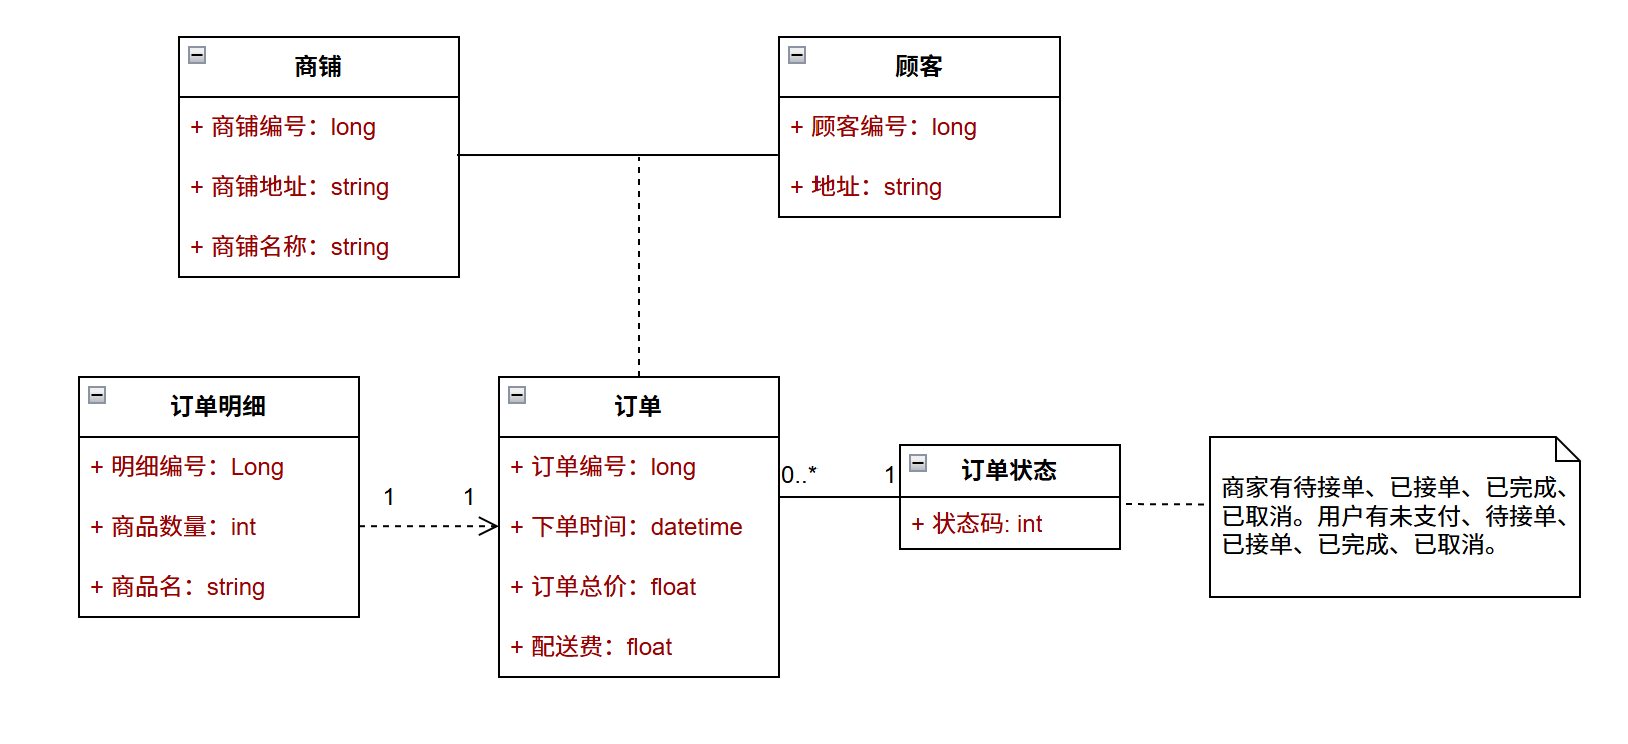
\includegraphics[width=5.80556in,height=2.61319in]{figures/srs/image3.png}
\caption{订单类图}
\changedfigure{需增加骑手、配送任务、订单状态历史、优惠核销、钱包支付、积分和评价关联。}
\end{figure}

(2) 用户基本信息

\begin{figure}[htbp]
\centering
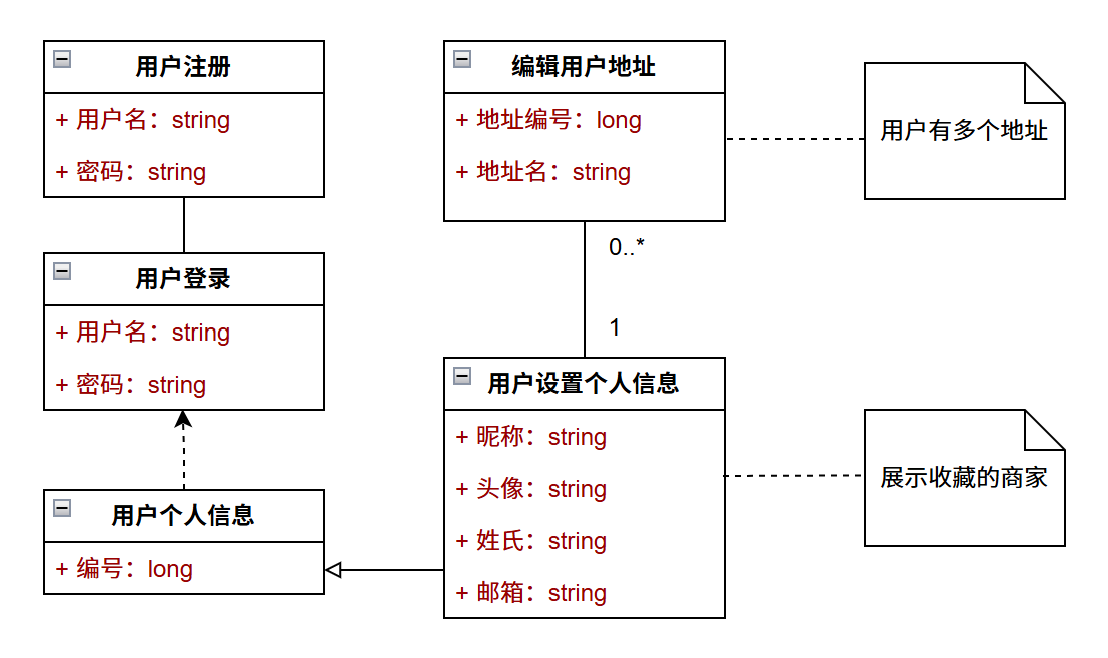
\includegraphics[width=5.59167in,height=3.06806in]{figures/srs/image4.png}
\caption{用户类图}
\changedfigure{需增加 RIDER 角色、骑手资料、主题与口味偏好、钱包、积分和会员关系。}
\end{figure}

(4) 商品管理

\begin{figure}[htbp]
\centering
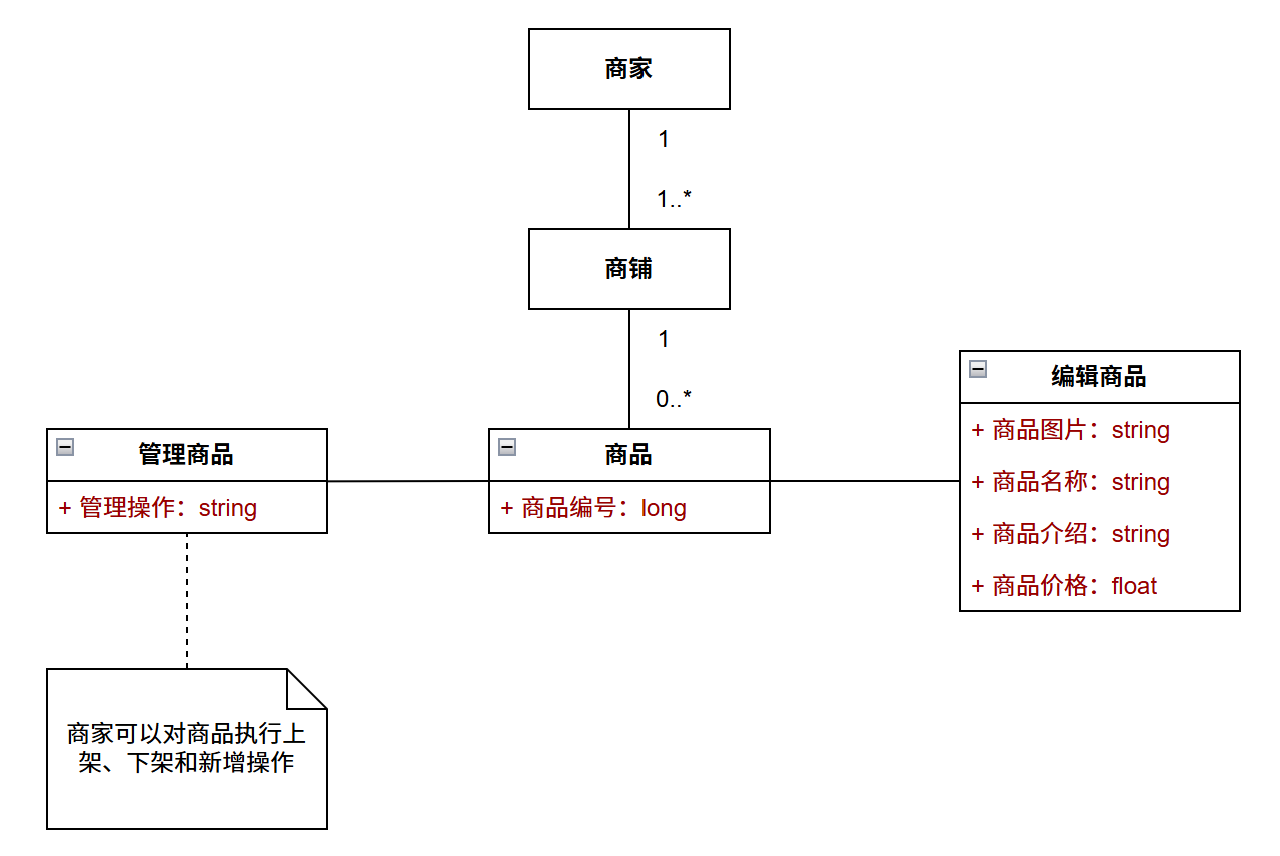
\includegraphics[width=5.69861in,height=3.86181in]{figures/srs/image5.png}
\caption{商品管理类图}
\changedfigure{需增加库存、月售、热销排名、折扣、限购、促销活动、评论和推荐特征。}
\end{figure}

(4) 商铺管理

\begin{figure}[htbp]
\centering
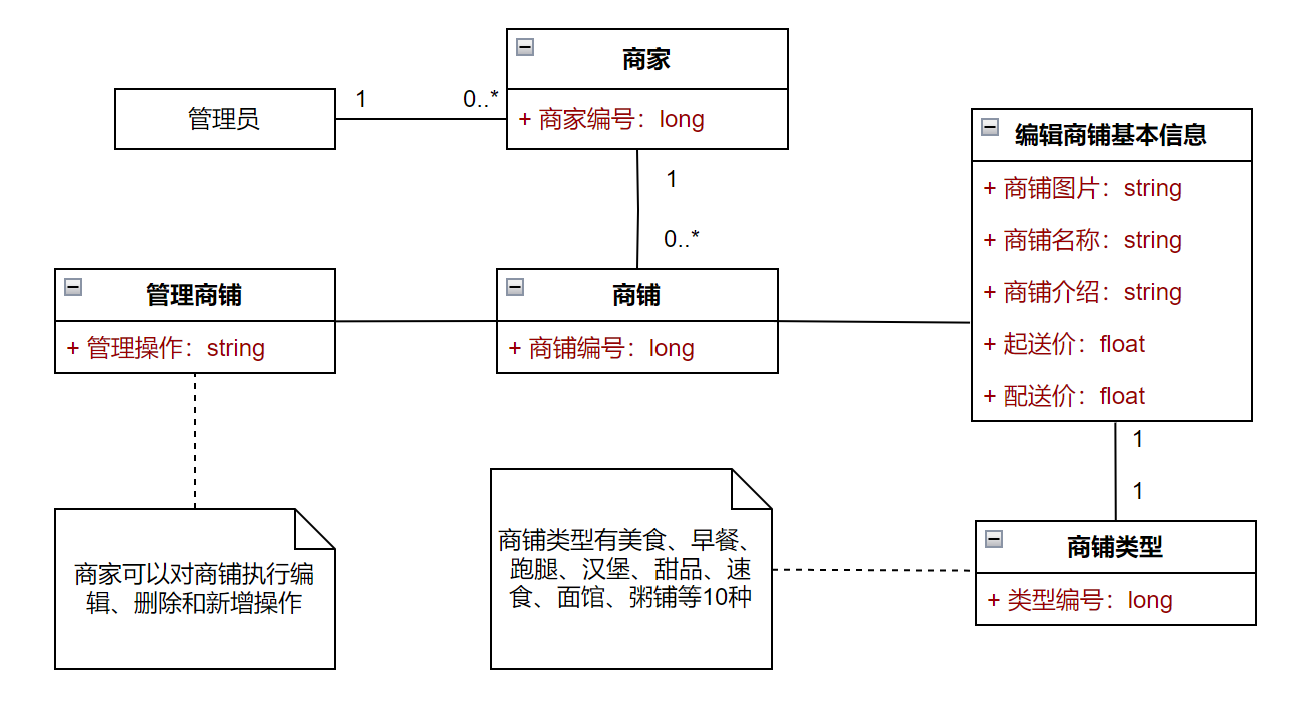
\includegraphics[width=5.37153in,height=2.96111in]{figures/srs/image6.png}
\caption{商铺管理类图}
\changedfigure{需增加营业/休息状态、商家故事、活动配置、配送配置和经营统计关系。}
\end{figure}

(5) 用户管理

\begin{figure}[htbp]
\centering
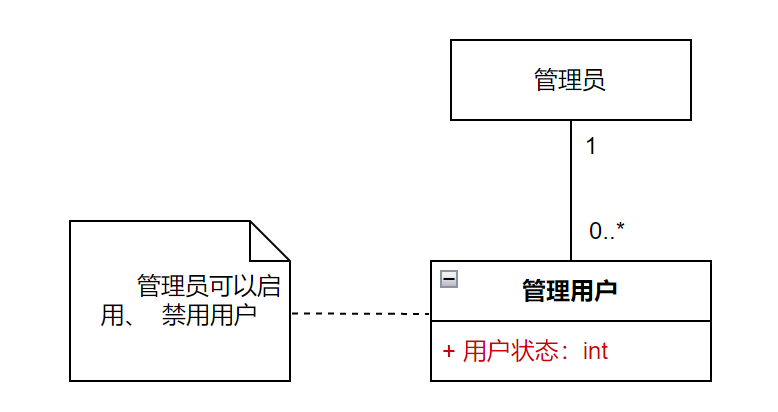
\includegraphics[width=2.86597in,height=1.51806in]{figures/srs/image7.png}
\caption{用户管理类图}
\changedfigure{需增加骑手审核、角色授权、账号状态、隐私范围和操作审计。}
\end{figure}

(6) 点赞收藏评分

\begin{figure}[htbp]
\centering
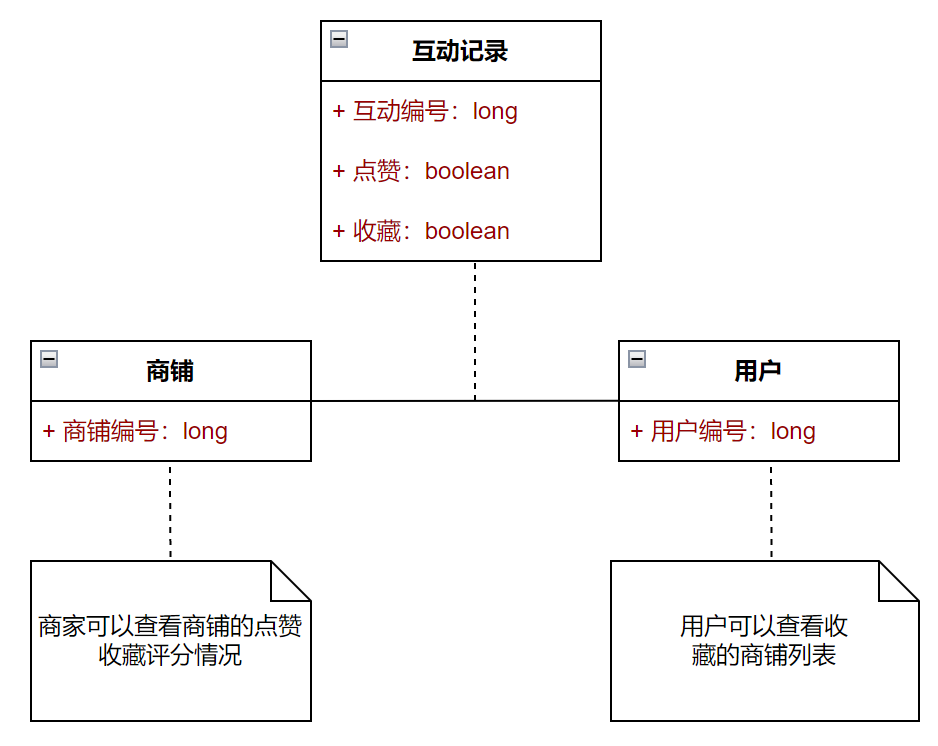
\includegraphics[width=3.37917in,height=2.68681in]{figures/srs/image8.png}
\caption{点赞收藏评分类图}
\changedfigure{需增加基于已完成订单的评价、评分、图片、商家回复、举报和管理员治理。}
\end{figure}

\subsection{业务流程分析 (UML活动图)}\label{ux4e1aux52a1ux6d41ux7a0bux5206ux6790-umlux6d3bux52a8ux56fe}

(1) 用户登录 \& 注册流程

\begin{figure}[htbp]
\centering
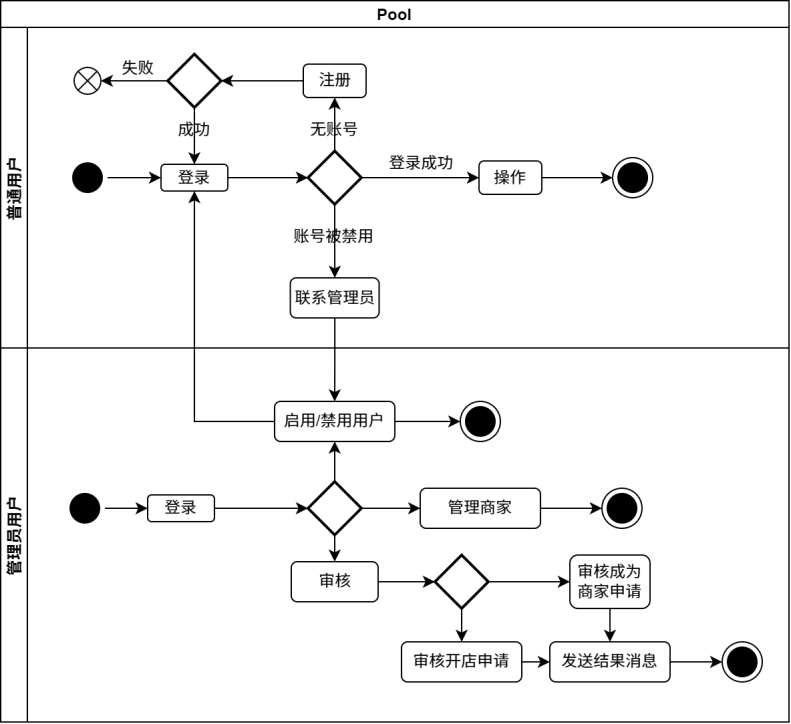
\includegraphics[width=3.59444in,height=3.29097in]{figures/srs/image9.png}
\caption{登录注册活动图}
\changedfigure{需增加骑手申请与审核、RIDER 权限、账号禁用校验及按角色进入不同工作台。}
\end{figure}

\textbf{(2) 订单处理流程}

\begin{figure}[htbp]
\centering
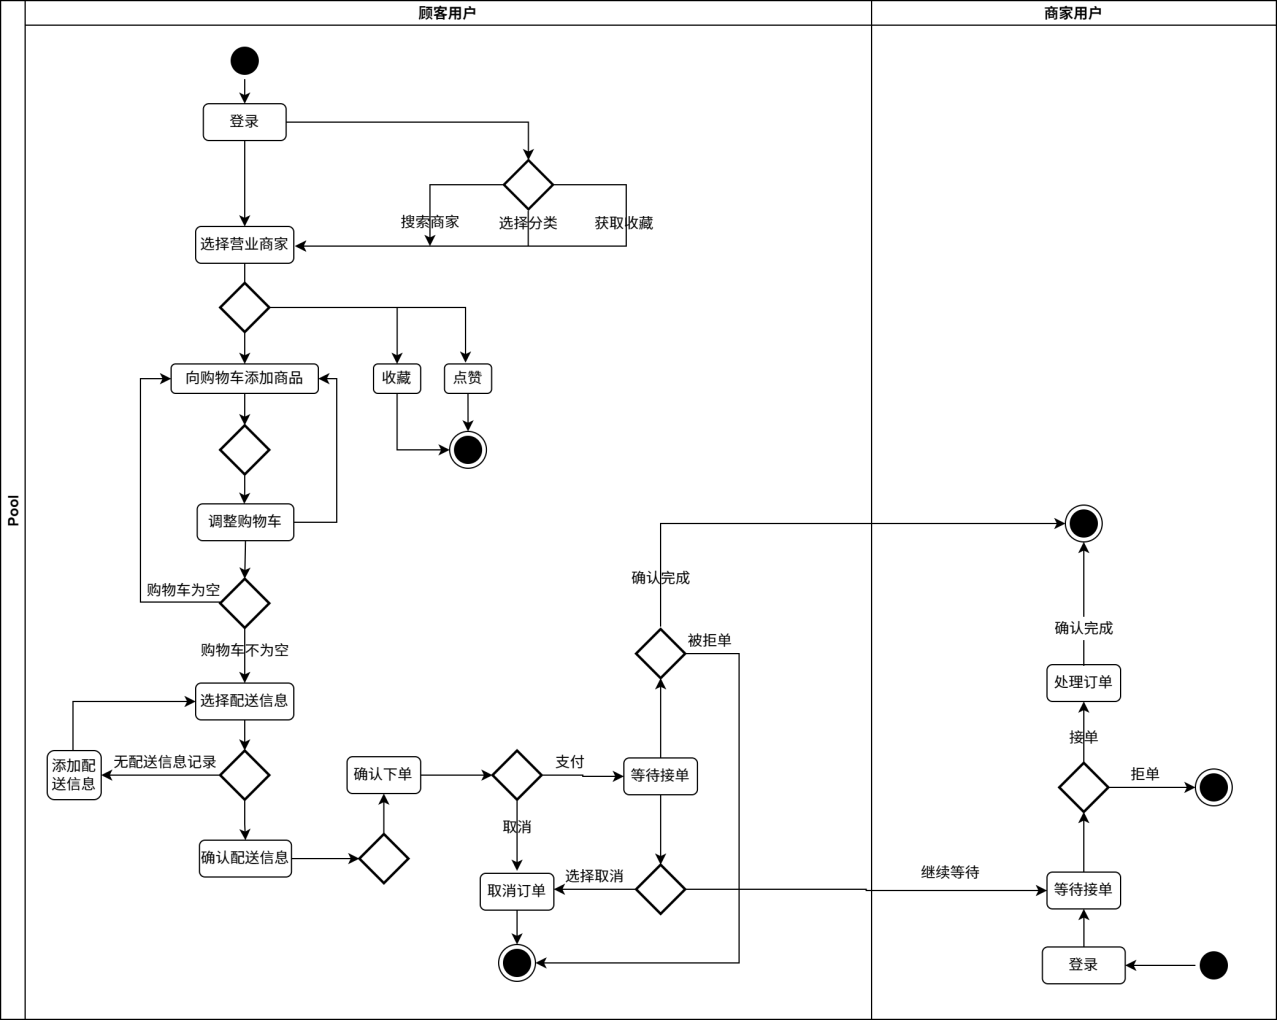
\includegraphics[width=5.80625in,height=4.63542in]{figures/srs/image10.png}
\caption{订单处理活动图}
\changedfigure{需加入优惠计算与核销、模拟钱包支付、派单/抢单、到店、取餐、配送、送达、异常和资产回退。}
\end{figure}

(3)商家管理流程

\begin{figure}[htbp]
\centering
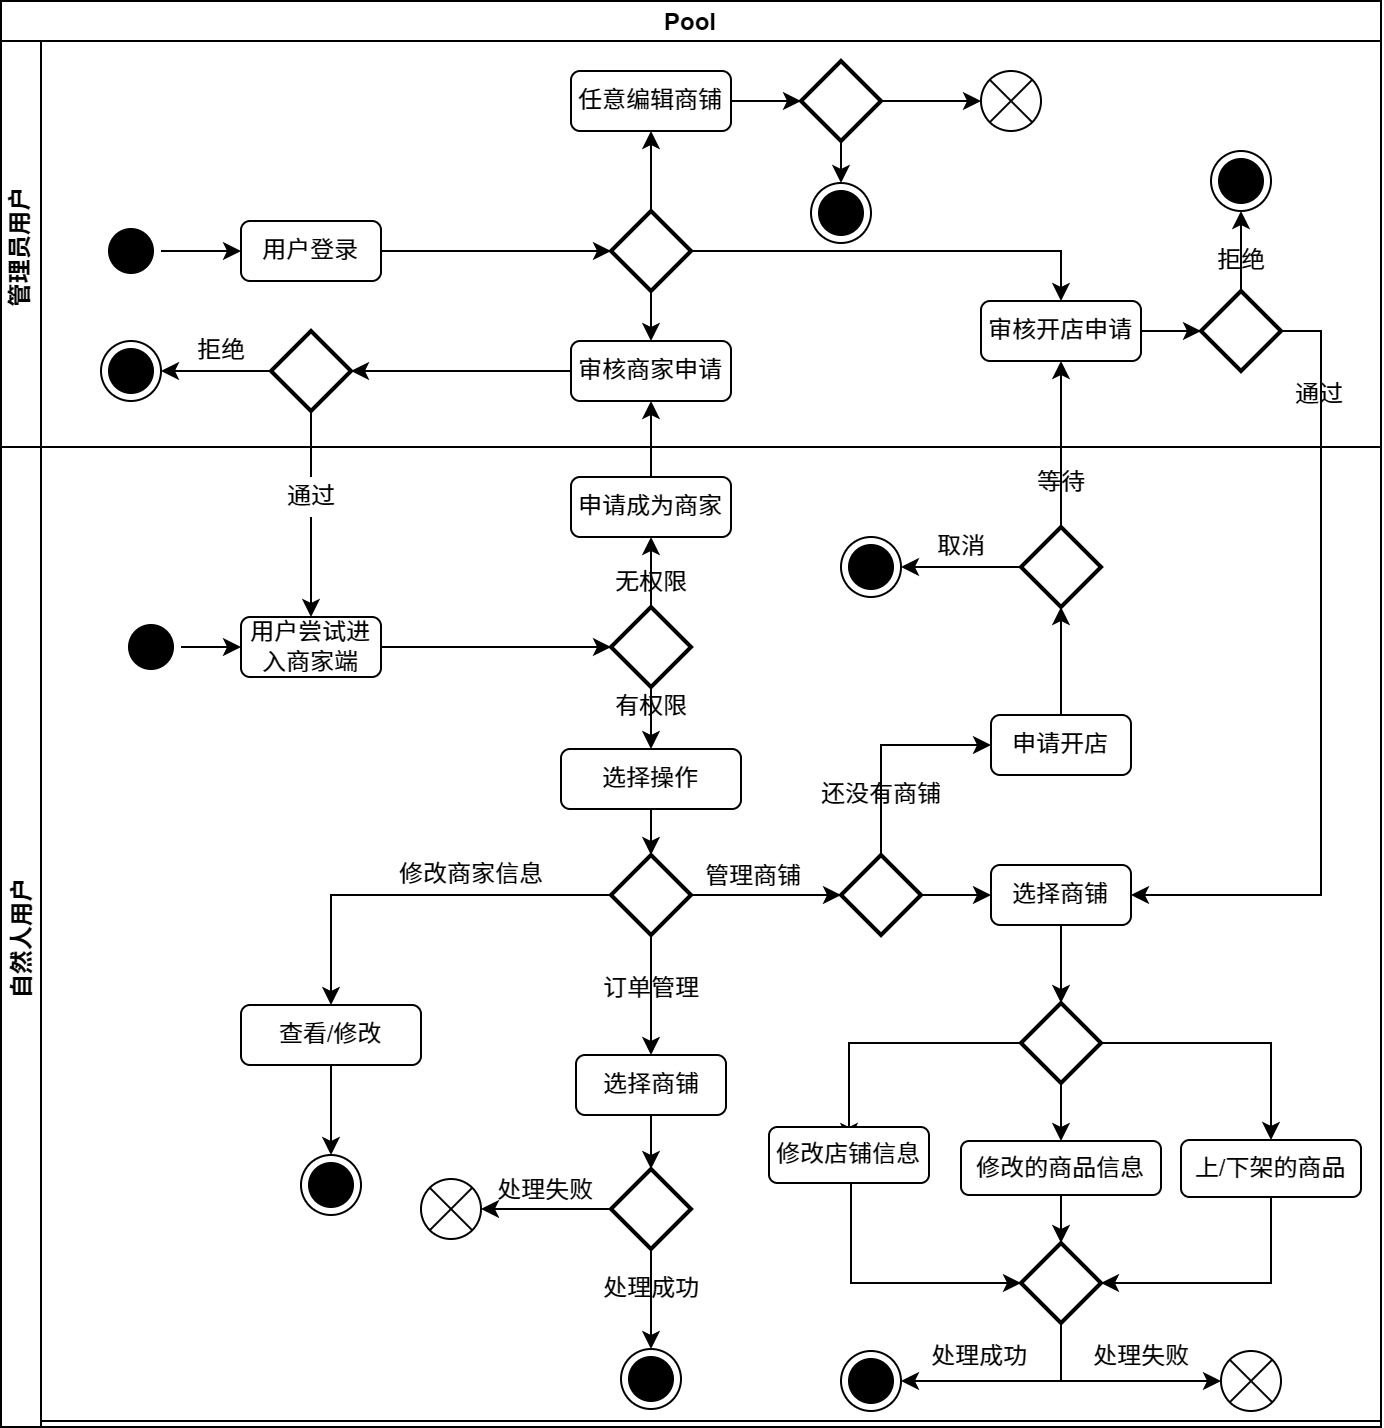
\includegraphics[width=5.84792in,height=6.03333in]{figures/srs/image11.png}
\caption{商家管理活动图}
\changedfigure{需加入商家故事、促销活动、商品折扣限购、经营看板以及与骑手的出餐交接。}
\end{figure}

\section{功能性需求}\label{ux529fux80fdux6027ux9700ux6c42}

\subsection{总用例}\label{ux603bux7528ux4f8b}

\begin{figure}[htbp]
\centering
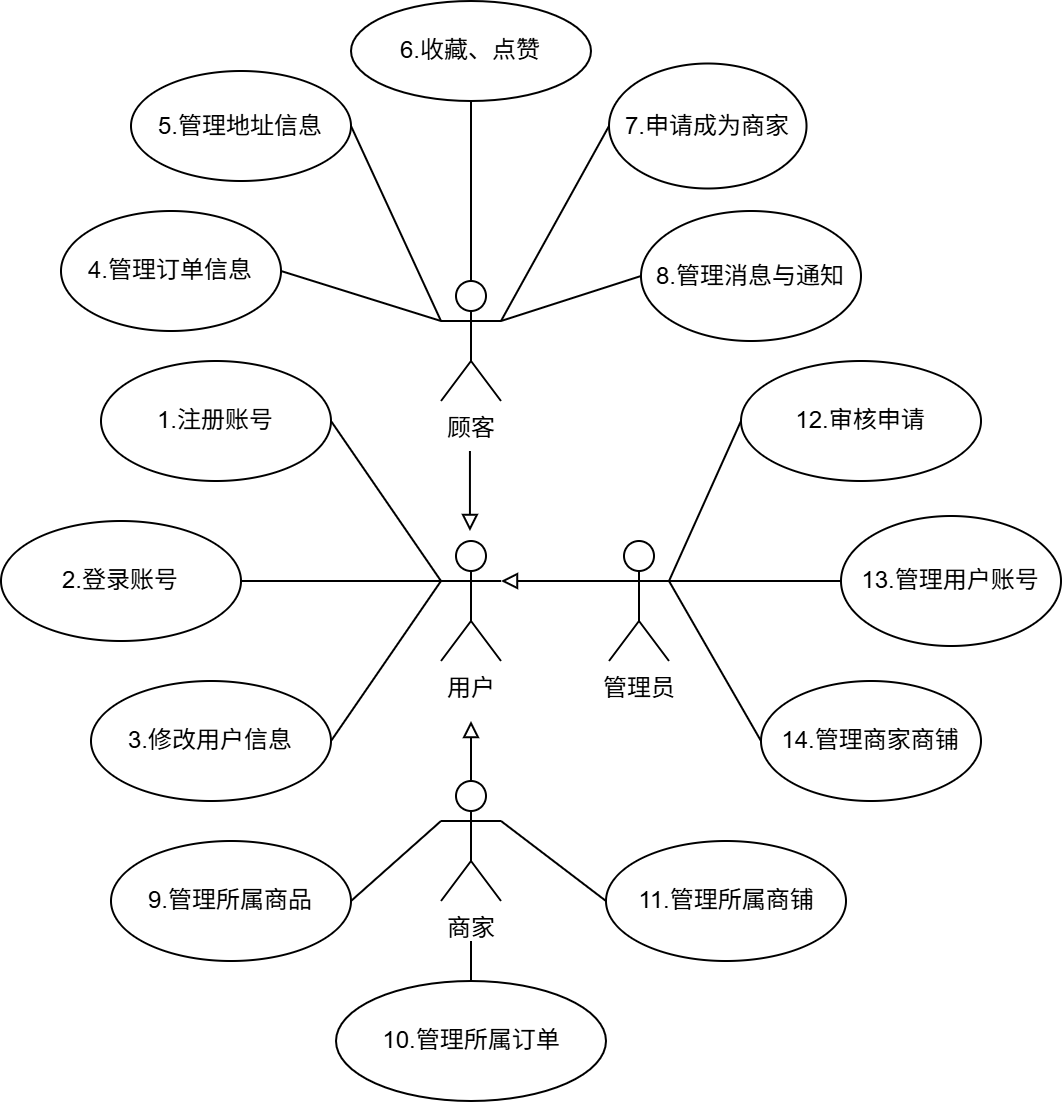
\includegraphics[width=4.18403in,height=4.34306in]{figures/srs/image12.png}
\caption{总用例图}
\changedfigure{需增加骑手参与者、外部地图/AI/语音/识图服务，以及营销资产、个性化、评价和看板用例。}
\end{figure}

\subsection{用户的用例}\label{ux7528ux6237ux7684ux7528ux4f8b}

\begin{figure}[htbp]
\centering
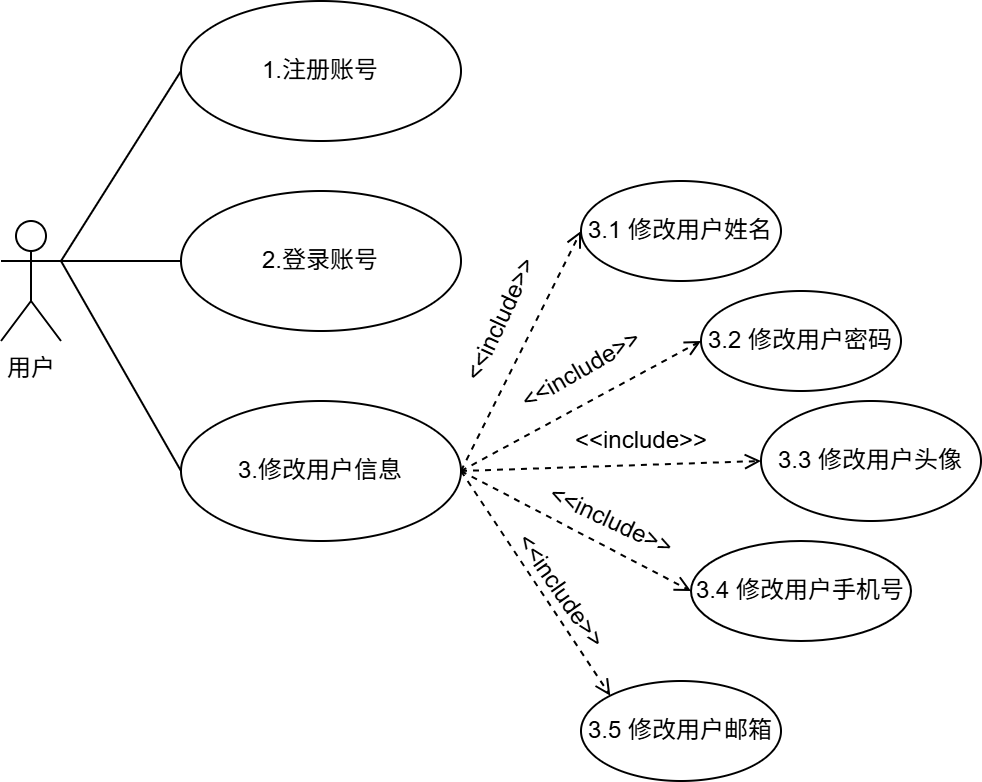
\includegraphics[width=4.31806in,height=3.43889in]{figures/srs/image13.png}
\caption{用户用例图}
\changedfigure{需增加骑手角色申请与工作台、主题偏好、钱包积分会员，以及多角色切换。}
\end{figure}

\begin{longtable}[]{@{}
  >{\centering\arraybackslash}p{(\linewidth - 8\tabcolsep) * \real{0.1614}}
  >{\centering\arraybackslash}p{(\linewidth - 8\tabcolsep) * \real{0.1672}}
  >{\centering\arraybackslash}p{(\linewidth - 8\tabcolsep) * \real{0.1304}}
  >{\centering\arraybackslash}p{(\linewidth - 8\tabcolsep) * \real{0.3716}}
  >{\centering\arraybackslash}p{(\linewidth - 8\tabcolsep) * \real{0.0027}}@{}}
\caption{注册账号用例说明}\tabularnewline
\toprule\noalign{}
\endfirsthead
\endhead
\bottomrule\noalign{}
\endlastfoot
\textbf{编号} & 1 & \textbf{名称} &
\multicolumn{2}{>{\centering\arraybackslash}p{(\linewidth - 8\tabcolsep) * \real{0.3743} + 2\tabcolsep}@{}}{%
注册账号} \\
\textbf{执行者} & 用户 & \textbf{优先级} &
\multicolumn{2}{>{\centering\arraybackslash}p{(\linewidth - 8\tabcolsep) * \real{0.3743} + 2\tabcolsep}@{}}{%
高} \\
\textbf{描述} &
\multicolumn{3}{>{\raggedright\arraybackslash}p{(\linewidth - 8\tabcolsep) * \real{0.6692} + 4\tabcolsep}}{%
用户使用用户名进行账户注册, 设置账户密码} & \\
\textbf{前置条件} &
\multicolumn{3}{>{\raggedright\arraybackslash}p{(\linewidth - 8\tabcolsep) * \real{0.6692} + 4\tabcolsep}}{%
该用户名未被注册} & \\
\textbf{基本流程} &
\multicolumn{3}{>{\raggedright\arraybackslash}p{(\linewidth - 8\tabcolsep) * \real{0.6692} + 4\tabcolsep}}{%
1. 输入用户名

2. 输入密码

3. 输入其他个人信息} & \\
\textbf{结束状况} &
\multicolumn{3}{>{\raggedright\arraybackslash}p{(\linewidth - 8\tabcolsep) * \real{0.6692} + 4\tabcolsep}}{%
注册成功进入首页} & \\
\textbf{可选流程} &
\multicolumn{3}{>{\raggedright\arraybackslash}p{(\linewidth - 8\tabcolsep) * \real{0.6692} + 4\tabcolsep}}{%
-} & \\
\textbf{异常流程} &
\multicolumn{3}{>{\raggedright\arraybackslash}p{(\linewidth - 8\tabcolsep) * \real{0.6692} + 4\tabcolsep}}{%
1.用户已经注册，显示用户已存在} & \\
\textbf{备注} &
\multicolumn{3}{>{\raggedright\arraybackslash}p{(\linewidth - 8\tabcolsep) * \real{0.6692} + 4\tabcolsep}}{%
用户注册后即拥有顾客权限} & \\
\end{longtable}

\begin{longtable}[]{@{}
  >{\centering\arraybackslash}p{(\linewidth - 6\tabcolsep) * \real{0.1690}}
  >{\centering\arraybackslash}p{(\linewidth - 6\tabcolsep) * \real{0.1685}}
  >{\centering\arraybackslash}p{(\linewidth - 6\tabcolsep) * \real{0.1350}}
  >{\centering\arraybackslash}p{(\linewidth - 6\tabcolsep) * \real{0.3572}}@{}}
\caption{登录账号用例说明}\tabularnewline
\toprule\noalign{}
\endfirsthead
\endhead
\bottomrule\noalign{}
\endlastfoot
\textbf{编号} & 2 & \textbf{名称} & 登录账号 \\
\textbf{执行者} & 用户 & \textbf{优先级} & 高 \\
\textbf{描述} &
\multicolumn{3}{>{\raggedright\arraybackslash}p{(\linewidth - 6\tabcolsep) * \real{0.6608} + 4\tabcolsep}@{}}{%
用户使用用户名密码进行账户登录} \\
\textbf{前置条件} &
\multicolumn{3}{>{\raggedright\arraybackslash}p{(\linewidth - 6\tabcolsep) * \real{0.6608} + 4\tabcolsep}@{}}{%
1. 提交正确的用户名

2. 提交正确的密码} \\
\textbf{基本流程} &
\multicolumn{3}{>{\raggedright\arraybackslash}p{(\linewidth - 6\tabcolsep) * \real{0.6608} + 4\tabcolsep}@{}}{%
1. 输入用户名

2. 输入密码

3. 显示登录成功信息} \\
\textbf{结束状况} &
\multicolumn{3}{>{\raggedright\arraybackslash}p{(\linewidth - 6\tabcolsep) * \real{0.6608} + 4\tabcolsep}@{}}{%
1. 登录成功后返回上一个页面

2. 登录成功后进入管理员首页} \\
\textbf{可选流程} &
\multicolumn{3}{>{\raggedright\arraybackslash}p{(\linewidth - 6\tabcolsep) * \real{0.6608} + 4\tabcolsep}@{}}{%
注册账号} \\
\textbf{异常流程} &
\multicolumn{3}{>{\raggedright\arraybackslash}p{(\linewidth - 6\tabcolsep) * \real{0.6608} + 4\tabcolsep}@{}}{%
1. 用户未注册进入用户注册流程

2. 密码验证不通过} \\
\textbf{备注} &
\multicolumn{3}{>{\raggedright\arraybackslash}p{(\linewidth - 6\tabcolsep) * \real{0.6608} + 4\tabcolsep}@{}}{%
\begin{minipage}[t]{\linewidth}\raggedright
\begin{quote}
只要该用户有管理员权限，登录后便进入管理端首

页否则进入顾客端首页
\end{quote}
\end{minipage}} \\
\end{longtable}

\begin{longtable}[]{@{}
  >{\centering\arraybackslash}p{(\linewidth - 6\tabcolsep) * \real{0.1690}}
  >{\centering\arraybackslash}p{(\linewidth - 6\tabcolsep) * \real{0.1685}}
  >{\centering\arraybackslash}p{(\linewidth - 6\tabcolsep) * \real{0.1350}}
  >{\centering\arraybackslash}p{(\linewidth - 6\tabcolsep) * \real{0.3572}}@{}}
\caption{修改用户信息用例说明}\tabularnewline
\toprule\noalign{}
\endfirsthead
\endhead
\bottomrule\noalign{}
\endlastfoot
\textbf{编号} & 3 & \textbf{名称} & 修改用户信息 \\
\textbf{执行者} & 用户 & \textbf{优先级} & 高 \\
\textbf{描述} &
\multicolumn{3}{>{\raggedright\arraybackslash}p{(\linewidth - 6\tabcolsep) * \real{0.6608} + 4\tabcolsep}@{}}{%
用户修改用户信息} \\
\textbf{前置条件} &
\multicolumn{3}{>{\raggedright\arraybackslash}p{(\linewidth - 6\tabcolsep) * \real{0.6608} + 4\tabcolsep}@{}}{%
1.用户已登录} \\
\textbf{基本流程} &
\multicolumn{3}{>{\raggedright\arraybackslash}p{(\linewidth - 6\tabcolsep) * \real{0.6608} + 4\tabcolsep}@{}}{%
1. 进入``我的''界面

2. 修改用户姓名、密码、头像、手机号、邮箱

3. 提交修改} \\
\textbf{结束状况} &
\multicolumn{3}{>{\raggedright\arraybackslash}p{(\linewidth - 6\tabcolsep) * \real{0.6608} + 4\tabcolsep}@{}}{%
1. 显示修改后的用户信息} \\
\textbf{可选流程} &
\multicolumn{3}{>{\raggedright\arraybackslash}p{(\linewidth - 6\tabcolsep) * \real{0.6608} + 4\tabcolsep}@{}}{%
} \\
\textbf{异常流程} &
\multicolumn{3}{>{\raggedright\arraybackslash}p{(\linewidth - 6\tabcolsep) * \real{0.6608} + 4\tabcolsep}@{}}{%
1. 用户修改后的手机号格式不符合规范

2. 用户修改后的邮箱格式不符合规范} \\
\textbf{备注} &
\multicolumn{3}{>{\raggedright\arraybackslash}p{(\linewidth - 6\tabcolsep) * \real{0.6608} + 4\tabcolsep}@{}}{%
-} \\
\end{longtable}

\subsection{顾客的用例}\label{ux987eux5ba2ux7684ux7528ux4f8b}

\begin{figure}[htbp]
\centering
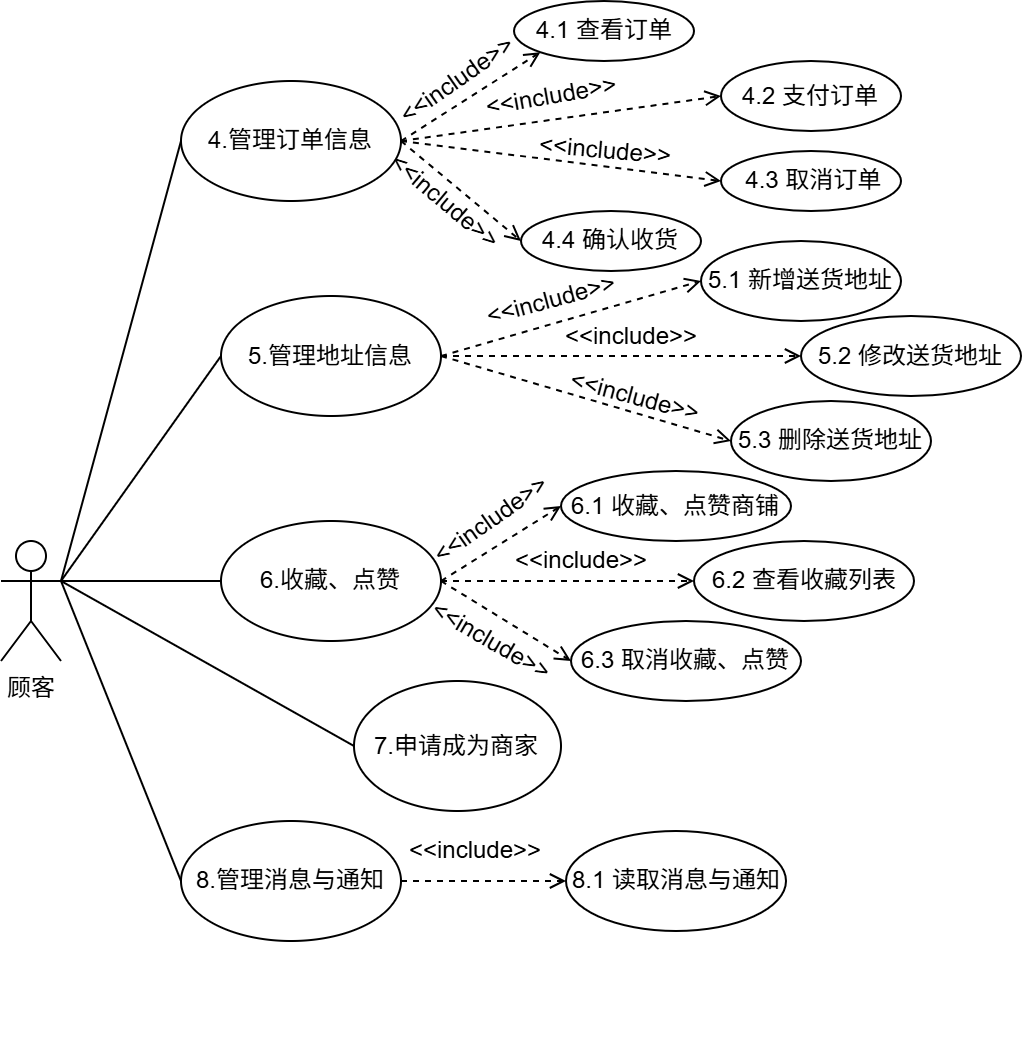
\includegraphics[width=5.19444in,height=4.87083in]{figures/srs/image14.png}
\caption{顾客用例图}
\changedfigure{需增加优惠与钱包支付、智能推荐/识图/语音、配送跟踪、订单评价和消费看板。}
\end{figure}

\begin{longtable}[]{@{}
  >{\centering\arraybackslash}p{(\linewidth - 6\tabcolsep) * \real{0.1720}}
  >{\centering\arraybackslash}p{(\linewidth - 6\tabcolsep) * \real{0.2080}}
  >{\centering\arraybackslash}p{(\linewidth - 6\tabcolsep) * \real{0.1810}}
  >{\centering\arraybackslash}p{(\linewidth - 6\tabcolsep) * \real{0.2687}}@{}}
\caption{查看订单说明}\tabularnewline
\toprule\noalign{}
\endfirsthead
\endhead
\bottomrule\noalign{}
\endlastfoot
\textbf{编号} & 4.1 & \textbf{名称} & 查看订单 \\
\textbf{执行者} & 顾客 & \textbf{优先级} & 低 \\
\textbf{描述} &
\multicolumn{3}{>{\raggedright\arraybackslash}p{(\linewidth - 6\tabcolsep) * \real{0.6577} + 4\tabcolsep}@{}}{%
顾客查看订单} \\
\textbf{前置条件} &
\multicolumn{3}{>{\raggedright\arraybackslash}p{(\linewidth - 6\tabcolsep) * \real{0.6577} + 4\tabcolsep}@{}}{%
无} \\
\textbf{基本流程} &
\multicolumn{3}{>{\raggedright\arraybackslash}p{(\linewidth - 6\tabcolsep) * \real{0.6577} + 4\tabcolsep}@{}}{%
1. 点击页面下方``订单''图标

2. 查看订单列表

3. 点击可查看订单详情} \\
\textbf{结束状况} &
\multicolumn{3}{>{\raggedright\arraybackslash}p{(\linewidth - 6\tabcolsep) * \real{0.6577} + 4\tabcolsep}@{}}{%
显示订单列表} \\
\textbf{可选流程} &
\multicolumn{3}{>{\raggedright\arraybackslash}p{(\linewidth - 6\tabcolsep) * \real{0.6577} + 4\tabcolsep}@{}}{%
顾客可以选择查看不同状态的订单列表：待支付、

待接单、已接单、已取消、已完成} \\
\textbf{异常流程} &
\multicolumn{3}{>{\raggedright\arraybackslash}p{(\linewidth - 6\tabcolsep) * \real{0.6577} + 4\tabcolsep}@{}}{%
-} \\
\textbf{备注} &
\multicolumn{3}{>{\raggedright\arraybackslash}p{(\linewidth - 6\tabcolsep) * \real{0.6577} + 4\tabcolsep}@{}}{%
-} \\
\end{longtable}

\begin{longtable}[]{@{}
  >{\centering\arraybackslash}p{(\linewidth - 6\tabcolsep) * \real{0.1541}}
  >{\centering\arraybackslash}p{(\linewidth - 6\tabcolsep) * \real{0.2036}}
  >{\centering\arraybackslash}p{(\linewidth - 6\tabcolsep) * \real{0.1904}}
  >{\centering\arraybackslash}p{(\linewidth - 6\tabcolsep) * \real{0.2816}}@{}}
\caption{支付订单说明}\tabularnewline
\toprule\noalign{}
\endfirsthead
\endhead
\bottomrule\noalign{}
\endlastfoot
\textbf{编号} & 4.2 & \textbf{名称} & 支付订单 \\
\textbf{执行者} & 顾客 & \textbf{优先级} & 低 \\
\textbf{描述} &
\multicolumn{3}{>{\raggedright\arraybackslash}p{(\linewidth - 6\tabcolsep) * \real{0.6756} + 4\tabcolsep}@{}}{%
顾客支付订单} \\
\textbf{前置条件} &
\multicolumn{3}{>{\raggedright\arraybackslash}p{(\linewidth - 6\tabcolsep) * \real{0.6756} + 4\tabcolsep}@{}}{%
顾客下单} \\
\textbf{基本流程} &
\multicolumn{3}{>{\raggedright\arraybackslash}p{(\linewidth - 6\tabcolsep) * \real{0.6756} + 4\tabcolsep}@{}}{%
1. 点击``去支付''按钮

2. 选择微信支付或者支付宝支付（默认）} \\
\textbf{结束状况} &
\multicolumn{3}{>{\raggedright\arraybackslash}p{(\linewidth - 6\tabcolsep) * \real{0.6756} + 4\tabcolsep}@{}}{%
订单已支付，状态变为待接单} \\
\textbf{可选流程} &
\multicolumn{3}{>{\raggedright\arraybackslash}p{(\linewidth - 6\tabcolsep) * \real{0.6756} + 4\tabcolsep}@{}}{%
-} \\
\textbf{异常流程} &
\multicolumn{3}{>{\raggedright\arraybackslash}p{(\linewidth - 6\tabcolsep) * \real{0.6756} + 4\tabcolsep}@{}}{%
-} \\
\textbf{备注} &
\multicolumn{3}{>{\raggedright\arraybackslash}p{(\linewidth - 6\tabcolsep) * \real{0.6756} + 4\tabcolsep}@{}}{%
-} \\
\end{longtable}

\begin{longtable}[]{@{}
  >{\centering\arraybackslash}p{(\linewidth - 6\tabcolsep) * \real{0.1884}}
  >{\centering\arraybackslash}p{(\linewidth - 6\tabcolsep) * \real{0.1986}}
  >{\centering\arraybackslash}p{(\linewidth - 6\tabcolsep) * \real{0.1939}}
  >{\centering\arraybackslash}p{(\linewidth - 6\tabcolsep) * \real{0.2487}}@{}}
\caption{取消订单说明}\tabularnewline
\toprule\noalign{}
\endfirsthead
\endhead
\bottomrule\noalign{}
\endlastfoot
\textbf{编号} & 4.3 & \textbf{名称} & 取消订单 \\
\textbf{执行者} & 顾客 & \textbf{优先级} & 低 \\
\textbf{描述} &
\multicolumn{3}{>{\raggedright\arraybackslash}p{(\linewidth - 6\tabcolsep) * \real{0.6413} + 4\tabcolsep}@{}}{%
顾客取消订单} \\
\textbf{前置条件} &
\multicolumn{3}{>{\raggedright\arraybackslash}p{(\linewidth - 6\tabcolsep) * \real{0.6413} + 4\tabcolsep}@{}}{%
订单未被商家接单} \\
\textbf{基本流程} &
\multicolumn{3}{>{\raggedright\arraybackslash}p{(\linewidth - 6\tabcolsep) * \real{0.6413} + 4\tabcolsep}@{}}{%
1. 顾客点击``取消订单''按钮

2. 在弹出的提示框中选择``确认''} \\
\textbf{结束状况} &
\multicolumn{3}{>{\raggedright\arraybackslash}p{(\linewidth - 6\tabcolsep) * \real{0.6413} + 4\tabcolsep}@{}}{%
订单状态变为已取消} \\
\textbf{可选流程} &
\multicolumn{3}{>{\raggedright\arraybackslash}p{(\linewidth - 6\tabcolsep) * \real{0.6413} + 4\tabcolsep}@{}}{%
-} \\
\textbf{异常流程} &
\multicolumn{3}{>{\raggedright\arraybackslash}p{(\linewidth - 6\tabcolsep) * \real{0.6413} + 4\tabcolsep}@{}}{%
订单已被商家接单，弹出提示框``订单已被接单，

不能取消！''} \\
\textbf{备注} &
\multicolumn{3}{>{\raggedright\arraybackslash}p{(\linewidth - 6\tabcolsep) * \real{0.6413} + 4\tabcolsep}@{}}{%
顾客取消订单后商家端该订单状态显示同步被修改

为``已取消''} \\
\end{longtable}

\begin{longtable}[]{@{}
  >{\centering\arraybackslash}p{(\linewidth - 6\tabcolsep) * \real{0.1721}}
  >{\centering\arraybackslash}p{(\linewidth - 6\tabcolsep) * \real{0.1993}}
  >{\centering\arraybackslash}p{(\linewidth - 6\tabcolsep) * \real{0.1768}}
  >{\centering\arraybackslash}p{(\linewidth - 6\tabcolsep) * \real{0.2815}}@{}}
\caption{确认收货说明}\tabularnewline
\toprule\noalign{}
\endfirsthead
\endhead
\bottomrule\noalign{}
\endlastfoot
\textbf{编号} & 4.4 & \textbf{名称} & 确认收货 \\
\textbf{执行者} & 顾客 & \textbf{优先级} & 低 \\
\textbf{描述} &
\multicolumn{3}{>{\raggedright\arraybackslash}p{(\linewidth - 6\tabcolsep) * \real{0.6576} + 4\tabcolsep}@{}}{%
顾客将订单状态改为已完成} \\
\textbf{前置条件} &
\multicolumn{3}{>{\raggedright\arraybackslash}p{(\linewidth - 6\tabcolsep) * \real{0.6576} + 4\tabcolsep}@{}}{%
订单已被商家接单} \\
\textbf{基本流程} &
\multicolumn{3}{>{\raggedright\arraybackslash}p{(\linewidth - 6\tabcolsep) * \real{0.6576} + 4\tabcolsep}@{}}{%
1. 点击``确认收货''按钮} \\
\textbf{结束状况} &
\multicolumn{3}{>{\raggedright\arraybackslash}p{(\linewidth - 6\tabcolsep) * \real{0.6576} + 4\tabcolsep}@{}}{%
订单状态变为已完成} \\
\textbf{可选流程} &
\multicolumn{3}{>{\raggedright\arraybackslash}p{(\linewidth - 6\tabcolsep) * \real{0.6576} + 4\tabcolsep}@{}}{%
-} \\
\textbf{异常流程} &
\multicolumn{3}{>{\raggedright\arraybackslash}p{(\linewidth - 6\tabcolsep) * \real{0.6576} + 4\tabcolsep}@{}}{%
-} \\
\textbf{备注} &
\multicolumn{3}{>{\raggedright\arraybackslash}p{(\linewidth - 6\tabcolsep) * \real{0.6576} + 4\tabcolsep}@{}}{%
\begin{minipage}[t]{\linewidth}\raggedright
\begin{quote}
顾客确认收货后商家端该订单状态显示同步被修改为``已完成''
\end{quote}
\end{minipage}} \\
\end{longtable}

\begin{longtable}[]{@{}
  >{\centering\arraybackslash}p{(\linewidth - 6\tabcolsep) * \real{0.1721}}
  >{\centering\arraybackslash}p{(\linewidth - 6\tabcolsep) * \real{0.2009}}
  >{\centering\arraybackslash}p{(\linewidth - 6\tabcolsep) * \real{0.1738}}
  >{\centering\arraybackslash}p{(\linewidth - 6\tabcolsep) * \real{0.2829}}@{}}
\caption{新增收货地址说明}\tabularnewline
\toprule\noalign{}
\endfirsthead
\endhead
\bottomrule\noalign{}
\endlastfoot
\textbf{编号} & 5.1 & \textbf{名称} & 新增送货地址 \\
\textbf{执行者} & 顾客 & \textbf{优先级} & 低 \\
\textbf{描述} &
\multicolumn{3}{>{\raggedright\arraybackslash}p{(\linewidth - 6\tabcolsep) * \real{0.6576} + 4\tabcolsep}@{}}{%
顾客新增地址列表中的送货地址} \\
\textbf{前置条件} &
\multicolumn{3}{>{\raggedright\arraybackslash}p{(\linewidth - 6\tabcolsep) * \real{0.6576} + 4\tabcolsep}@{}}{%
-} \\
\textbf{基本流程} &
\multicolumn{3}{>{\raggedright\arraybackslash}p{(\linewidth - 6\tabcolsep) * \real{0.6576} + 4\tabcolsep}@{}}{%
1. 点击地址界面的新建用户地址

2. 依次填入地址信息

3. 显示新建地址成功界面} \\
\textbf{结束状况} &
\multicolumn{3}{>{\raggedright\arraybackslash}p{(\linewidth - 6\tabcolsep) * \real{0.6576} + 4\tabcolsep}@{}}{%
地址列表出现新地址} \\
\textbf{可选流程} &
\multicolumn{3}{>{\raggedright\arraybackslash}p{(\linewidth - 6\tabcolsep) * \real{0.6576} + 4\tabcolsep}@{}}{%
1. 地址中的必填信息未填写，需要写入} \\
\textbf{异常流程} &
\multicolumn{3}{>{\raggedright\arraybackslash}p{(\linewidth - 6\tabcolsep) * \real{0.6576} + 4\tabcolsep}@{}}{%
-} \\
\textbf{备注} &
\multicolumn{3}{>{\raggedright\arraybackslash}p{(\linewidth - 6\tabcolsep) * \real{0.6576} + 4\tabcolsep}@{}}{%
-} \\
\end{longtable}

\begin{longtable}[]{@{}
  >{\centering\arraybackslash}p{(\linewidth - 6\tabcolsep) * \real{0.1723}}
  >{\centering\arraybackslash}p{(\linewidth - 6\tabcolsep) * \real{0.2009}}
  >{\centering\arraybackslash}p{(\linewidth - 6\tabcolsep) * \real{0.1795}}
  >{\centering\arraybackslash}p{(\linewidth - 6\tabcolsep) * \real{0.2949}}@{}}
\caption{修改收货地址说明}\tabularnewline
\toprule\noalign{}
\endfirsthead
\endhead
\bottomrule\noalign{}
\endlastfoot
\textbf{编号} & 5.2 & \textbf{名称} & 修改送货地址 \\
\textbf{执行者} & 顾客 & \textbf{优先级} & 低 \\
\textbf{描述} &
\multicolumn{3}{>{\raggedright\arraybackslash}p{(\linewidth - 6\tabcolsep) * \real{0.6752} + 4\tabcolsep}@{}}{%
顾客修改地址列表中的送货地址} \\
\textbf{前置条件} &
\multicolumn{3}{>{\raggedright\arraybackslash}p{(\linewidth - 6\tabcolsep) * \real{0.6752} + 4\tabcolsep}@{}}{%
-} \\
\textbf{基本流程} &
\multicolumn{3}{>{\raggedright\arraybackslash}p{(\linewidth - 6\tabcolsep) * \real{0.6752} + 4\tabcolsep}@{}}{%
1. 点击地址界面的用户地址

2. 修改地址信息

3. 显示修改地址成功界面} \\
\textbf{结束状况} &
\multicolumn{3}{>{\raggedright\arraybackslash}p{(\linewidth - 6\tabcolsep) * \real{0.6752} + 4\tabcolsep}@{}}{%
地址列表出现修改后的新地址} \\
\textbf{可选流程} &
\multicolumn{3}{>{\raggedright\arraybackslash}p{(\linewidth - 6\tabcolsep) * \real{0.6752} + 4\tabcolsep}@{}}{%
地址中的必填信息未填写，需要写入} \\
\textbf{异常流程} &
\multicolumn{3}{>{\raggedright\arraybackslash}p{(\linewidth - 6\tabcolsep) * \real{0.6752} + 4\tabcolsep}@{}}{%
-} \\
\textbf{备注} &
\multicolumn{3}{>{\raggedright\arraybackslash}p{(\linewidth - 6\tabcolsep) * \real{0.6752} + 4\tabcolsep}@{}}{%
-} \\
\end{longtable}

\begin{longtable}[]{@{}
  >{\centering\arraybackslash}p{(\linewidth - 6\tabcolsep) * \real{0.1723}}
  >{\centering\arraybackslash}p{(\linewidth - 6\tabcolsep) * \real{0.2009}}
  >{\centering\arraybackslash}p{(\linewidth - 6\tabcolsep) * \real{0.1795}}
  >{\centering\arraybackslash}p{(\linewidth - 6\tabcolsep) * \real{0.2949}}@{}}
\caption{删除收货地址说明}\tabularnewline
\toprule\noalign{}
\endfirsthead
\endhead
\bottomrule\noalign{}
\endlastfoot
\textbf{编号} & 5.3 & \textbf{名称} & 删除送货地址 \\
\textbf{执行者} & 顾客 & \textbf{优先级} & 低 \\
\textbf{描述} &
\multicolumn{3}{>{\raggedright\arraybackslash}p{(\linewidth - 6\tabcolsep) * \real{0.6752} + 4\tabcolsep}@{}}{%
顾客删除地址列表中的送货地址} \\
\textbf{前置条件} &
\multicolumn{3}{>{\raggedright\arraybackslash}p{(\linewidth - 6\tabcolsep) * \real{0.6752} + 4\tabcolsep}@{}}{%
地址列表中有已经存在的地址} \\
\textbf{基本流程} &
\multicolumn{3}{>{\raggedright\arraybackslash}p{(\linewidth - 6\tabcolsep) * \real{0.6752} + 4\tabcolsep}@{}}{%
1. 点击地址界面的用户地址，进入用户的地址列表面

2. 选中需要删除的地址，点击删除，询问是否删除

3. 显示删除地址成功界面} \\
\textbf{结束状况} &
\multicolumn{3}{>{\raggedright\arraybackslash}p{(\linewidth - 6\tabcolsep) * \real{0.6752} + 4\tabcolsep}@{}}{%
用户的地址列表界面原地址消失} \\
\textbf{可选流程} &
\multicolumn{3}{>{\raggedright\arraybackslash}p{(\linewidth - 6\tabcolsep) * \real{0.6752} + 4\tabcolsep}@{}}{%
\begin{minipage}[t]{\linewidth}\raggedright
\begin{quote}
误触点到删除，询问是否删除时点击否，返回用户地址列表界面
\end{quote}
\end{minipage}} \\
\textbf{异常流程} &
\multicolumn{3}{>{\raggedright\arraybackslash}p{(\linewidth - 6\tabcolsep) * \real{0.6752} + 4\tabcolsep}@{}}{%
} \\
\textbf{备注} &
\multicolumn{3}{>{\raggedright\arraybackslash}p{(\linewidth - 6\tabcolsep) * \real{0.6752} + 4\tabcolsep}@{}}{%
} \\
\end{longtable}

\begin{longtable}[]{@{}
  >{\centering\arraybackslash}p{(\linewidth - 6\tabcolsep) * \real{0.1622}}
  >{\centering\arraybackslash}p{(\linewidth - 6\tabcolsep) * \real{0.2009}}
  >{\centering\arraybackslash}p{(\linewidth - 6\tabcolsep) * \real{0.1809}}
  >{\centering\arraybackslash}p{(\linewidth - 6\tabcolsep) * \real{0.2857}}@{}}
\caption{收藏点赞店铺说明}\tabularnewline
\toprule\noalign{}
\endfirsthead
\endhead
\bottomrule\noalign{}
\endlastfoot
\textbf{编号} & 6.1 & \textbf{名称} & 收藏、点赞商铺 \\
\textbf{执行者} & 顾客 & \textbf{优先级} & 低 \\
\textbf{描述} &
\multicolumn{3}{>{\raggedright\arraybackslash}p{(\linewidth - 6\tabcolsep) * \real{0.6675} + 4\tabcolsep}@{}}{%
顾客收藏、点赞商铺} \\
\textbf{前置条件} &
\multicolumn{3}{>{\raggedright\arraybackslash}p{(\linewidth - 6\tabcolsep) * \real{0.6675} + 4\tabcolsep}@{}}{%
无} \\
\textbf{基本流程} &
\multicolumn{3}{>{\raggedright\arraybackslash}p{(\linewidth - 6\tabcolsep) * \real{0.6675} + 4\tabcolsep}@{}}{%
1. 进入商铺

2. 点击收藏或点赞按钮} \\
\textbf{结束状况} &
\multicolumn{3}{>{\raggedright\arraybackslash}p{(\linewidth - 6\tabcolsep) * \real{0.6675} + 4\tabcolsep}@{}}{%
收藏或点赞按钮被点亮} \\
\textbf{可选流程} &
\multicolumn{3}{>{\raggedright\arraybackslash}p{(\linewidth - 6\tabcolsep) * \real{0.6675} + 4\tabcolsep}@{}}{%
-} \\
\textbf{异常流程} &
\multicolumn{3}{>{\raggedright\arraybackslash}p{(\linewidth - 6\tabcolsep) * \real{0.6675} + 4\tabcolsep}@{}}{%
-} \\
\textbf{备注} &
\multicolumn{3}{>{\raggedright\arraybackslash}p{(\linewidth - 6\tabcolsep) * \real{0.6675} + 4\tabcolsep}@{}}{%
-} \\
\end{longtable}

\begin{longtable}[]{@{}
  >{\centering\arraybackslash}p{(\linewidth - 6\tabcolsep) * \real{0.1608}}
  >{\centering\arraybackslash}p{(\linewidth - 6\tabcolsep) * \real{0.2023}}
  >{\centering\arraybackslash}p{(\linewidth - 6\tabcolsep) * \real{0.1809}}
  >{\centering\arraybackslash}p{(\linewidth - 6\tabcolsep) * \real{0.2857}}@{}}
\caption{查看收藏列表说明}\tabularnewline
\toprule\noalign{}
\endfirsthead
\endhead
\bottomrule\noalign{}
\endlastfoot
\textbf{编号} & 6.2 & \textbf{名称} & 查看收藏列表 \\
\textbf{执行者} & 顾客 & \textbf{优先级} & 低 \\
\textbf{描述} &
\multicolumn{3}{>{\raggedright\arraybackslash}p{(\linewidth - 6\tabcolsep) * \real{0.6689} + 4\tabcolsep}@{}}{%
顾客查看收藏列表} \\
\textbf{前置条件} &
\multicolumn{3}{>{\raggedright\arraybackslash}p{(\linewidth - 6\tabcolsep) * \real{0.6689} + 4\tabcolsep}@{}}{%
无} \\
\textbf{基本流程} &
\multicolumn{3}{>{\raggedright\arraybackslash}p{(\linewidth - 6\tabcolsep) * \real{0.6689} + 4\tabcolsep}@{}}{%
1. 进入``我的''界面

2. 点击我的收藏

3. 查看收藏的所有商铺，点击可进入} \\
\textbf{结束状况} &
\multicolumn{3}{>{\raggedright\arraybackslash}p{(\linewidth - 6\tabcolsep) * \real{0.6689} + 4\tabcolsep}@{}}{%
-} \\
\textbf{可选流程} &
\multicolumn{3}{>{\raggedright\arraybackslash}p{(\linewidth - 6\tabcolsep) * \real{0.6689} + 4\tabcolsep}@{}}{%
-} \\
\textbf{异常流程} &
\multicolumn{3}{>{\raggedright\arraybackslash}p{(\linewidth - 6\tabcolsep) * \real{0.6689} + 4\tabcolsep}@{}}{%
-} \\
\textbf{备注} &
\multicolumn{3}{>{\raggedright\arraybackslash}p{(\linewidth - 6\tabcolsep) * \real{0.6689} + 4\tabcolsep}@{}}{%
-} \\
\end{longtable}

\begin{longtable}[]{@{}
  >{\centering\arraybackslash}p{(\linewidth - 6\tabcolsep) * \real{0.1541}}
  >{\centering\arraybackslash}p{(\linewidth - 6\tabcolsep) * \real{0.2104}}
  >{\centering\arraybackslash}p{(\linewidth - 6\tabcolsep) * \real{0.1809}}
  >{\centering\arraybackslash}p{(\linewidth - 6\tabcolsep) * \real{0.2843}}@{}}
\caption{取消点赞收藏说明}\tabularnewline
\toprule\noalign{}
\endfirsthead
\endhead
\bottomrule\noalign{}
\endlastfoot
\textbf{编号} & 6.3 & \textbf{名称} & 取消收藏、点赞 \\
\textbf{执行者} & 顾客 & \textbf{优先级} & 低 \\
\textbf{描述} &
\multicolumn{3}{>{\raggedright\arraybackslash}p{(\linewidth - 6\tabcolsep) * \real{0.6756} + 4\tabcolsep}@{}}{%
顾客取消收藏、点赞} \\
\textbf{前置条件} &
\multicolumn{3}{>{\raggedright\arraybackslash}p{(\linewidth - 6\tabcolsep) * \real{0.6756} + 4\tabcolsep}@{}}{%
无} \\
\textbf{基本流程} &
\multicolumn{3}{>{\raggedright\arraybackslash}p{(\linewidth - 6\tabcolsep) * \real{0.6756} + 4\tabcolsep}@{}}{%
1. 进入商铺

2. 再次点击收藏或点赞按钮} \\
\textbf{结束状况} &
\multicolumn{3}{>{\raggedright\arraybackslash}p{(\linewidth - 6\tabcolsep) * \real{0.6756} + 4\tabcolsep}@{}}{%
\begin{minipage}[t]{\linewidth}\raggedright
\begin{quote}
收藏或点赞按钮变暗，取消收藏后该店铺不再出现在我的收藏
\end{quote}
\end{minipage}} \\
\textbf{可选流程} &
\multicolumn{3}{>{\raggedright\arraybackslash}p{(\linewidth - 6\tabcolsep) * \real{0.6756} + 4\tabcolsep}@{}}{%
-} \\
\textbf{异常流程} &
\multicolumn{3}{>{\raggedright\arraybackslash}p{(\linewidth - 6\tabcolsep) * \real{0.6756} + 4\tabcolsep}@{}}{%
-} \\
\textbf{备注} &
\multicolumn{3}{>{\raggedright\arraybackslash}p{(\linewidth - 6\tabcolsep) * \real{0.6756} + 4\tabcolsep}@{}}{%
-} \\
\end{longtable}

\begin{longtable}[]{@{}
  >{\centering\arraybackslash}p{(\linewidth - 6\tabcolsep) * \real{0.1541}}
  >{\centering\arraybackslash}p{(\linewidth - 6\tabcolsep) * \real{0.2076}}
  >{\centering\arraybackslash}p{(\linewidth - 6\tabcolsep) * \real{0.1823}}
  >{\centering\arraybackslash}p{(\linewidth - 6\tabcolsep) * \real{0.2857}}@{}}
\caption{申请成为商家说明}\tabularnewline
\toprule\noalign{}
\endfirsthead
\endhead
\bottomrule\noalign{}
\endlastfoot
\textbf{编号} & 7 & \textbf{名称} & 申请成为商家 \\
\textbf{执行者} & 顾客 & \textbf{优先级} & 低 \\
\textbf{描述} &
\multicolumn{3}{>{\raggedright\arraybackslash}p{(\linewidth - 6\tabcolsep) * \real{0.6756} + 4\tabcolsep}@{}}{%
顾客申请成为商家} \\
\textbf{前置条件} &
\multicolumn{3}{>{\raggedright\arraybackslash}p{(\linewidth - 6\tabcolsep) * \real{0.6756} + 4\tabcolsep}@{}}{%
无} \\
\textbf{基本流程} &
\multicolumn{3}{>{\raggedright\arraybackslash}p{(\linewidth - 6\tabcolsep) * \real{0.6756} + 4\tabcolsep}@{}}{%
1. 进入``我的''页面

2. 点击申请成为商家按钮} \\
\textbf{结束状况} &
\multicolumn{3}{>{\raggedright\arraybackslash}p{(\linewidth - 6\tabcolsep) * \real{0.6756} + 4\tabcolsep}@{}}{%
管理端用户审核列表出现新条目，等待管理员审核} \\
\textbf{可选流程} &
\multicolumn{3}{>{\raggedright\arraybackslash}p{(\linewidth - 6\tabcolsep) * \real{0.6756} + 4\tabcolsep}@{}}{%
-} \\
\textbf{异常流程} &
\multicolumn{3}{>{\raggedright\arraybackslash}p{(\linewidth - 6\tabcolsep) * \real{0.6756} + 4\tabcolsep}@{}}{%
重复申请} \\
\textbf{备注} &
\multicolumn{3}{>{\raggedright\arraybackslash}p{(\linewidth - 6\tabcolsep) * \real{0.6756} + 4\tabcolsep}@{}}{%
-} \\
\end{longtable}

\begin{longtable}[]{@{}
  >{\centering\arraybackslash}p{(\linewidth - 6\tabcolsep) * \real{0.1541}}
  >{\centering\arraybackslash}p{(\linewidth - 6\tabcolsep) * \real{0.2076}}
  >{\centering\arraybackslash}p{(\linewidth - 6\tabcolsep) * \real{0.1809}}
  >{\centering\arraybackslash}p{(\linewidth - 6\tabcolsep) * \real{0.2871}}@{}}
\caption{读取消息通知说明}\tabularnewline
\toprule\noalign{}
\endfirsthead
\endhead
\bottomrule\noalign{}
\endlastfoot
\textbf{编号} & 8.1 & \textbf{名称} & 读取消息与通知 \\
\textbf{执行者} & 顾客 & \textbf{优先级} & 低 \\
\textbf{描述} &
\multicolumn{3}{>{\raggedright\arraybackslash}p{(\linewidth - 6\tabcolsep) * \real{0.6756} + 4\tabcolsep}@{}}{%
顾客读取消息与通知} \\
\textbf{前置条件} &
\multicolumn{3}{>{\raggedright\arraybackslash}p{(\linewidth - 6\tabcolsep) * \real{0.6756} + 4\tabcolsep}@{}}{%
无} \\
\textbf{基本流程} &
\multicolumn{3}{>{\raggedright\arraybackslash}p{(\linewidth - 6\tabcolsep) * \real{0.6756} + 4\tabcolsep}@{}}{%
1. 进入``我的''页面

2. 点击消息与通知

3. 点击待读取的消息} \\
\textbf{结束状况} &
\multicolumn{3}{>{\raggedright\arraybackslash}p{(\linewidth - 6\tabcolsep) * \real{0.6756} + 4\tabcolsep}@{}}{%
读取后消息与通知红点消失，消息由蓝色变为灰色} \\
\textbf{可选流程} &
\multicolumn{3}{>{\raggedright\arraybackslash}p{(\linewidth - 6\tabcolsep) * \real{0.6756} + 4\tabcolsep}@{}}{%
-} \\
\textbf{异常流程} &
\multicolumn{3}{>{\raggedright\arraybackslash}p{(\linewidth - 6\tabcolsep) * \real{0.6756} + 4\tabcolsep}@{}}{%
-} \\
\textbf{备注} &
\multicolumn{3}{>{\raggedright\arraybackslash}p{(\linewidth - 6\tabcolsep) * \real{0.6756} + 4\tabcolsep}@{}}{%
-} \\
\end{longtable}

\subsection{商家的用例}\label{ux5546ux5bb6ux7684ux7528ux4f8b}

\begin{figure}[htbp]
\centering
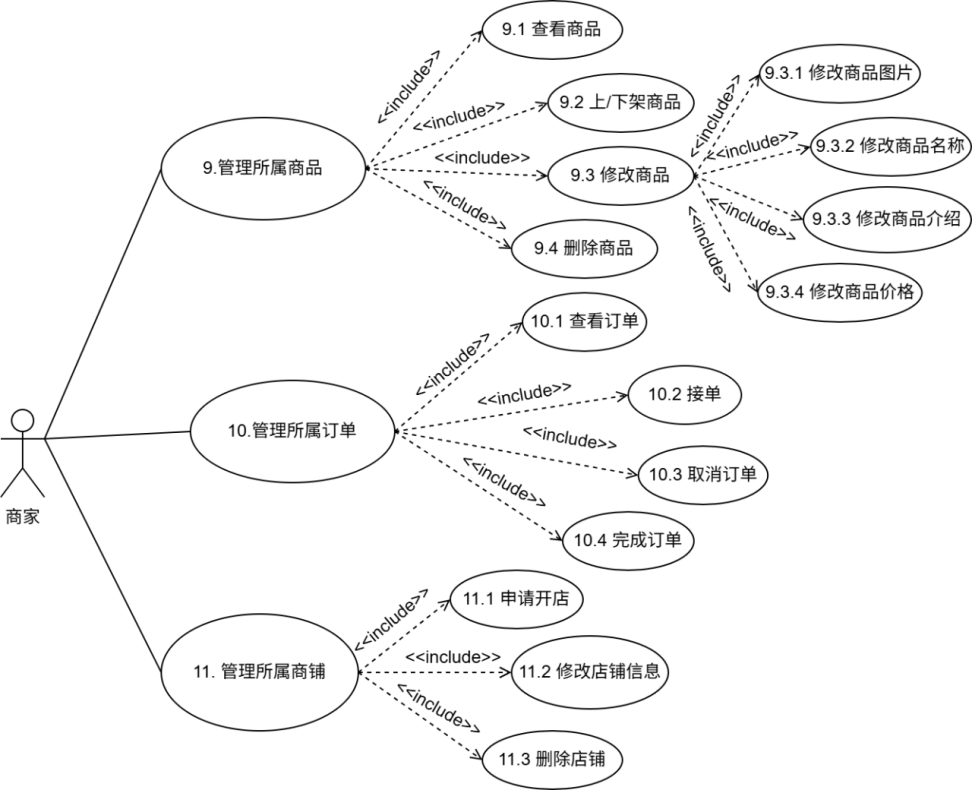
\includegraphics[width=5.78125in,height=4.69792in]{figures/srs/image15.png}
\caption{商家用例图}
\changedfigure{需增加出餐与骑手交接、促销、折扣限购、商家故事、评价回复和经营看板；商家不得越级完成配送订单。}
\end{figure}

\begin{longtable}[]{@{}
  >{\centering\arraybackslash}p{(\linewidth - 6\tabcolsep) * \real{0.1888}}
  >{\centering\arraybackslash}p{(\linewidth - 6\tabcolsep) * \real{0.1881}}
  >{\centering\arraybackslash}p{(\linewidth - 6\tabcolsep) * \real{0.1667}}
  >{\centering\arraybackslash}p{(\linewidth - 6\tabcolsep) * \real{0.2856}}@{}}
\caption{查看商品说明}\tabularnewline
\toprule\noalign{}
\endfirsthead
\endhead
\bottomrule\noalign{}
\endlastfoot
\textbf{编号} & 9.1 & \textbf{名称} & 查看商品 \\
\textbf{执行者} & 商家 & \textbf{优先级} & 低 \\
\textbf{描述} &
\multicolumn{3}{>{\centering\arraybackslash}p{(\linewidth - 6\tabcolsep) * \real{0.6403} + 4\tabcolsep}@{}}{%
商家查看所售商品} \\
\textbf{前置条件} &
\multicolumn{3}{>{\centering\arraybackslash}p{(\linewidth - 6\tabcolsep) * \real{0.6403} + 4\tabcolsep}@{}}{%
无} \\
\textbf{基本流程} &
\multicolumn{3}{>{\raggedright\arraybackslash}p{(\linewidth - 6\tabcolsep) * \real{0.6403} + 4\tabcolsep}@{}}{%
1. 点击页面下方``商铺''图标

2. 点击对应商铺的``编辑''按钮} \\
\textbf{结束状况} &
\multicolumn{3}{>{\raggedright\arraybackslash}p{(\linewidth - 6\tabcolsep) * \real{0.6403} + 4\tabcolsep}@{}}{%
显示该商铺的所有商品} \\
\textbf{可选流程} &
\multicolumn{3}{>{\raggedright\arraybackslash}p{(\linewidth - 6\tabcolsep) * \real{0.6403} + 4\tabcolsep}@{}}{%
-} \\
\textbf{异常流程} &
\multicolumn{3}{>{\raggedright\arraybackslash}p{(\linewidth - 6\tabcolsep) * \real{0.6403} + 4\tabcolsep}@{}}{%
-} \\
\textbf{备注} &
\multicolumn{3}{>{\raggedright\arraybackslash}p{(\linewidth - 6\tabcolsep) * \real{0.6403} + 4\tabcolsep}@{}}{%
-} \\
\end{longtable}

\begin{longtable}[]{@{}
  >{\centering\arraybackslash}p{(\linewidth - 6\tabcolsep) * \real{0.1888}}
  >{\centering\arraybackslash}p{(\linewidth - 6\tabcolsep) * \real{0.1881}}
  >{\centering\arraybackslash}p{(\linewidth - 6\tabcolsep) * \real{0.1667}}
  >{\centering\arraybackslash}p{(\linewidth - 6\tabcolsep) * \real{0.2856}}@{}}
\caption{上下架商品说明}\tabularnewline
\toprule\noalign{}
\endfirsthead
\endhead
\bottomrule\noalign{}
\endlastfoot
\textbf{编号} & 9.2 & \textbf{名称} & 上/下架商品 \\
\textbf{执行者} & 商家 & \textbf{优先级} & 低 \\
\textbf{描述} &
\multicolumn{3}{>{\raggedright\arraybackslash}p{(\linewidth - 6\tabcolsep) * \real{0.6403} + 4\tabcolsep}@{}}{%
商家上/下架商品} \\
\textbf{前置条件} &
\multicolumn{3}{>{\raggedright\arraybackslash}p{(\linewidth - 6\tabcolsep) * \real{0.6403} + 4\tabcolsep}@{}}{%
无} \\
\textbf{基本流程} &
\multicolumn{3}{>{\raggedright\arraybackslash}p{(\linewidth - 6\tabcolsep) * \real{0.6403} + 4\tabcolsep}@{}}{%
1. 进入对应商铺

2. 点击对应商品的``上架/下架''按钮} \\
\textbf{结束状况} &
\multicolumn{3}{>{\raggedright\arraybackslash}p{(\linewidth - 6\tabcolsep) * \real{0.6403} + 4\tabcolsep}@{}}{%
\begin{minipage}[t]{\linewidth}\raggedright
\begin{quote}
下架商品，则该商品条目名称下方出现``已下架''上架商品，则该商品条目恢复原状
\end{quote}
\end{minipage}} \\
\textbf{可选流程} &
\multicolumn{3}{>{\raggedright\arraybackslash}p{(\linewidth - 6\tabcolsep) * \real{0.6403} + 4\tabcolsep}@{}}{%
-} \\
\textbf{异常流程} &
\multicolumn{3}{>{\raggedright\arraybackslash}p{(\linewidth - 6\tabcolsep) * \real{0.6403} + 4\tabcolsep}@{}}{%
-} \\
\textbf{备注} &
\multicolumn{3}{>{\raggedright\arraybackslash}p{(\linewidth - 6\tabcolsep) * \real{0.6403} + 4\tabcolsep}@{}}{%
-} \\
\end{longtable}

\begin{longtable}[]{@{}
  >{\centering\arraybackslash}p{(\linewidth - 6\tabcolsep) * \real{0.1888}}
  >{\centering\arraybackslash}p{(\linewidth - 6\tabcolsep) * \real{0.1882}}
  >{\centering\arraybackslash}p{(\linewidth - 6\tabcolsep) * \real{0.1681}}
  >{\centering\arraybackslash}p{(\linewidth - 6\tabcolsep) * \real{0.2841}}@{}}
\caption{修改商品说明}\tabularnewline
\toprule\noalign{}
\endfirsthead
\endhead
\bottomrule\noalign{}
\endlastfoot
\textbf{编号} & 9.3 & \textbf{名称} & 修改商品 \\
\textbf{执行者} & 商家 & \textbf{优先级} & 低 \\
\textbf{描述} &
\multicolumn{3}{>{\raggedright\arraybackslash}p{(\linewidth - 6\tabcolsep) * \real{0.6403} + 4\tabcolsep}@{}}{%
商家修改商品} \\
\textbf{前置条件} &
\multicolumn{3}{>{\raggedright\arraybackslash}p{(\linewidth - 6\tabcolsep) * \real{0.6403} + 4\tabcolsep}@{}}{%
无} \\
\textbf{基本流程} &
\multicolumn{3}{>{\raggedright\arraybackslash}p{(\linewidth - 6\tabcolsep) * \real{0.6403} + 4\tabcolsep}@{}}{%
1. 进入对应商铺

2. 点击对应商品的``编辑''按钮

3. 输入商品修改后的信息} \\
\textbf{结束状况} &
\multicolumn{3}{>{\raggedright\arraybackslash}p{(\linewidth - 6\tabcolsep) * \real{0.6403} + 4\tabcolsep}@{}}{%
商铺详情页面显示修改后的商品} \\
\textbf{可选流程} &
\multicolumn{3}{>{\raggedright\arraybackslash}p{(\linewidth - 6\tabcolsep) * \real{0.6403} + 4\tabcolsep}@{}}{%
-} \\
\textbf{异常流程} &
\multicolumn{3}{>{\raggedright\arraybackslash}p{(\linewidth - 6\tabcolsep) * \real{0.6403} + 4\tabcolsep}@{}}{%
-} \\
\textbf{备注} &
\multicolumn{3}{>{\raggedright\arraybackslash}p{(\linewidth - 6\tabcolsep) * \real{0.6403} + 4\tabcolsep}@{}}{%
修改项包括修改商品图片、名称、介绍、价格} \\
\end{longtable}

\begin{longtable}[]{@{}
  >{\centering\arraybackslash}p{(\linewidth - 6\tabcolsep) * \real{0.1888}}
  >{\centering\arraybackslash}p{(\linewidth - 6\tabcolsep) * \real{0.2167}}
  >{\centering\arraybackslash}p{(\linewidth - 6\tabcolsep) * \real{0.1865}}
  >{\centering\arraybackslash}p{(\linewidth - 6\tabcolsep) * \real{0.2371}}@{}}
\caption{删除商品说明}\tabularnewline
\toprule\noalign{}
\endfirsthead
\endhead
\bottomrule\noalign{}
\endlastfoot
\textbf{编号} & 9.4 & \textbf{名称} & 删除商品 \\
\textbf{执行者} & 商家 & \textbf{优先级} & 低 \\
\textbf{描述} &
\multicolumn{3}{>{\raggedright\arraybackslash}p{(\linewidth - 6\tabcolsep) * \real{0.6403} + 4\tabcolsep}@{}}{%
商家删除商品} \\
\textbf{前置条件} &
\multicolumn{3}{>{\raggedright\arraybackslash}p{(\linewidth - 6\tabcolsep) * \real{0.6403} + 4\tabcolsep}@{}}{%
无} \\
\textbf{基本流程} &
\multicolumn{3}{>{\raggedright\arraybackslash}p{(\linewidth - 6\tabcolsep) * \real{0.6403} + 4\tabcolsep}@{}}{%
1. 进入对应商铺

2. 点击对应商品的``删除''按钮

3. 输入商品修改后的信息} \\
\textbf{结束状况} &
\multicolumn{3}{>{\raggedright\arraybackslash}p{(\linewidth - 6\tabcolsep) * \real{0.6403} + 4\tabcolsep}@{}}{%
商铺详情页面显示修改后的商品} \\
\textbf{可选流程} &
\multicolumn{3}{>{\raggedright\arraybackslash}p{(\linewidth - 6\tabcolsep) * \real{0.6403} + 4\tabcolsep}@{}}{%
-} \\
\textbf{异常流程} &
\multicolumn{3}{>{\raggedright\arraybackslash}p{(\linewidth - 6\tabcolsep) * \real{0.6403} + 4\tabcolsep}@{}}{%
-} \\
\textbf{备注} &
\multicolumn{3}{>{\raggedright\arraybackslash}p{(\linewidth - 6\tabcolsep) * \real{0.6403} + 4\tabcolsep}@{}}{%
修改项包括修改商品图片、名称、介绍、价格} \\
\end{longtable}

\begin{longtable}[]{@{}
  >{\centering\arraybackslash}p{(\linewidth - 6\tabcolsep) * \real{0.1888}}
  >{\centering\arraybackslash}p{(\linewidth - 6\tabcolsep) * \real{0.2181}}
  >{\centering\arraybackslash}p{(\linewidth - 6\tabcolsep) * \real{0.1851}}
  >{\centering\arraybackslash}p{(\linewidth - 6\tabcolsep) * \real{0.2371}}@{}}
\caption{查看订单说明}\tabularnewline
\toprule\noalign{}
\endfirsthead
\endhead
\bottomrule\noalign{}
\endlastfoot
\textbf{编号} & 10.1 & \textbf{名称} & 查看订单 \\
\textbf{执行者} & 商家 & \textbf{优先级} & 低 \\
\textbf{描述} &
\multicolumn{3}{>{\raggedright\arraybackslash}p{(\linewidth - 6\tabcolsep) * \real{0.6403} + 4\tabcolsep}@{}}{%
商家查看本商户的订单} \\
\textbf{前置条件} &
\multicolumn{3}{>{\raggedright\arraybackslash}p{(\linewidth - 6\tabcolsep) * \real{0.6403} + 4\tabcolsep}@{}}{%
无} \\
\textbf{基本流程} &
\multicolumn{3}{>{\raggedright\arraybackslash}p{(\linewidth - 6\tabcolsep) * \real{0.6403} + 4\tabcolsep}@{}}{%
1. 进入商家``订单''页面

2. 选择对应商铺} \\
\textbf{结束状况} &
\multicolumn{3}{>{\raggedright\arraybackslash}p{(\linewidth - 6\tabcolsep) * \real{0.6403} + 4\tabcolsep}@{}}{%
显示商家该商铺不同状态的订单列表} \\
\textbf{可选流程} &
\multicolumn{3}{>{\raggedright\arraybackslash}p{(\linewidth - 6\tabcolsep) * \real{0.6403} + 4\tabcolsep}@{}}{%
-} \\
\textbf{异常流程} &
\multicolumn{3}{>{\raggedright\arraybackslash}p{(\linewidth - 6\tabcolsep) * \real{0.6403} + 4\tabcolsep}@{}}{%
-} \\
\textbf{备注} &
\multicolumn{3}{>{\raggedright\arraybackslash}p{(\linewidth - 6\tabcolsep) * \real{0.6403} + 4\tabcolsep}@{}}{%
\begin{minipage}[t]{\linewidth}\raggedright
\begin{quote}
商家端显示的订单状态分为：待接单、已接单、已取消、已完成
\end{quote}
\end{minipage}} \\
\end{longtable}

\begin{longtable}[]{@{}
  >{\centering\arraybackslash}p{(\linewidth - 6\tabcolsep) * \real{0.1888}}
  >{\centering\arraybackslash}p{(\linewidth - 6\tabcolsep) * \real{0.2067}}
  >{\centering\arraybackslash}p{(\linewidth - 6\tabcolsep) * \real{0.1837}}
  >{\centering\arraybackslash}p{(\linewidth - 6\tabcolsep) * \real{0.2499}}@{}}
\caption{接单说明}\tabularnewline
\toprule\noalign{}
\endfirsthead
\endhead
\bottomrule\noalign{}
\endlastfoot
\textbf{编号} & 10.2 & \textbf{名称} & 接单 \\
\textbf{执行者} & 商家 & \textbf{优先级} & 低 \\
\textbf{描述} &
\multicolumn{3}{>{\raggedright\arraybackslash}p{(\linewidth - 6\tabcolsep) * \real{0.6403} + 4\tabcolsep}@{}}{%
商家接单} \\
\textbf{前置条件} &
\multicolumn{3}{>{\raggedright\arraybackslash}p{(\linewidth - 6\tabcolsep) * \real{0.6403} + 4\tabcolsep}@{}}{%
无} \\
\textbf{基本流程} &
\multicolumn{3}{>{\raggedright\arraybackslash}p{(\linewidth - 6\tabcolsep) * \real{0.6403} + 4\tabcolsep}@{}}{%
1. 进入商家``订单''页面，选择对应商铺

2. 选择查看``待接单''订单列表

3. 点击``接单''按钮} \\
\textbf{结束状况} &
\multicolumn{3}{>{\raggedright\arraybackslash}p{(\linewidth - 6\tabcolsep) * \real{0.6403} + 4\tabcolsep}@{}}{%
该订单从``待接单''状态转为``已接单''状态} \\
\textbf{可选流程} &
\multicolumn{3}{>{\raggedright\arraybackslash}p{(\linewidth - 6\tabcolsep) * \real{0.6403} + 4\tabcolsep}@{}}{%
-} \\
\textbf{异常流程} &
\multicolumn{3}{>{\raggedright\arraybackslash}p{(\linewidth - 6\tabcolsep) * \real{0.6403} + 4\tabcolsep}@{}}{%
-} \\
\textbf{备注} &
\multicolumn{3}{>{\raggedright\arraybackslash}p{(\linewidth - 6\tabcolsep) * \real{0.6403} + 4\tabcolsep}@{}}{%
\begin{minipage}[t]{\linewidth}\raggedright
\begin{quote}
当顾客支付订单后对应商家的待接单列表增加该订单；商家接单后顾客订单状态显示同步修改为``已接单''
\end{quote}
\end{minipage}} \\
\end{longtable}

\begin{longtable}[]{@{}
  >{\centering\arraybackslash}p{(\linewidth - 6\tabcolsep) * \real{0.1888}}
  >{\centering\arraybackslash}p{(\linewidth - 6\tabcolsep) * \real{0.2067}}
  >{\centering\arraybackslash}p{(\linewidth - 6\tabcolsep) * \real{0.1823}}
  >{\centering\arraybackslash}p{(\linewidth - 6\tabcolsep) * \real{0.2513}}@{}}
\caption{取消订单说明}\tabularnewline
\toprule\noalign{}
\endfirsthead
\endhead
\bottomrule\noalign{}
\endlastfoot
\textbf{编号} & 10.3 & \textbf{名称} & 取消订单 \\
\textbf{执行者} & 商家 & \textbf{优先级} & 低 \\
\textbf{描述} &
\multicolumn{3}{>{\raggedright\arraybackslash}p{(\linewidth - 6\tabcolsep) * \real{0.6403} + 4\tabcolsep}@{}}{%
商家取消订单} \\
\textbf{前置条件} &
\multicolumn{3}{>{\raggedright\arraybackslash}p{(\linewidth - 6\tabcolsep) * \real{0.6403} + 4\tabcolsep}@{}}{%
无} \\
\textbf{基本流程} &
\multicolumn{3}{>{\raggedright\arraybackslash}p{(\linewidth - 6\tabcolsep) * \real{0.6403} + 4\tabcolsep}@{}}{%
1. 进入商家``订单''页面，选择对应商铺

2. 选择查看``待接单''订单列表

3. 点击``取消''按钮} \\
\textbf{结束状况} &
\multicolumn{3}{>{\raggedright\arraybackslash}p{(\linewidth - 6\tabcolsep) * \real{0.6403} + 4\tabcolsep}@{}}{%
该订单从``待接单''状态转为``已取消''状态} \\
\textbf{可选流程} &
\multicolumn{3}{>{\raggedright\arraybackslash}p{(\linewidth - 6\tabcolsep) * \real{0.6403} + 4\tabcolsep}@{}}{%
-} \\
\textbf{异常流程} &
\multicolumn{3}{>{\raggedright\arraybackslash}p{(\linewidth - 6\tabcolsep) * \real{0.6403} + 4\tabcolsep}@{}}{%
-} \\
\textbf{备注} &
\multicolumn{3}{>{\raggedright\arraybackslash}p{(\linewidth - 6\tabcolsep) * \real{0.6403} + 4\tabcolsep}@{}}{%
仅商家接单前可以取消订单} \\
\end{longtable}

\begin{longtable}[]{@{}
  >{\centering\arraybackslash}p{(\linewidth - 6\tabcolsep) * \real{0.1888}}
  >{\centering\arraybackslash}p{(\linewidth - 6\tabcolsep) * \real{0.1996}}
  >{\centering\arraybackslash}p{(\linewidth - 6\tabcolsep) * \real{0.1724}}
  >{\centering\arraybackslash}p{(\linewidth - 6\tabcolsep) * \real{0.2683}}@{}}
\caption{完成订单说明}\tabularnewline
\toprule\noalign{}
\endfirsthead
\endhead
\bottomrule\noalign{}
\endlastfoot
\textbf{编号} & 10.4 & \textbf{名称} & 完成订单 \\
\textbf{执行者} & 商家 & \textbf{优先级} & 低 \\
\textbf{描述} &
\multicolumn{3}{>{\raggedright\arraybackslash}p{(\linewidth - 6\tabcolsep) * \real{0.6403} + 4\tabcolsep}@{}}{%
商家完成订单} \\
\textbf{前置条件} &
\multicolumn{3}{>{\raggedright\arraybackslash}p{(\linewidth - 6\tabcolsep) * \real{0.6403} + 4\tabcolsep}@{}}{%
无} \\
\textbf{基本流程} &
\multicolumn{3}{>{\raggedright\arraybackslash}p{(\linewidth - 6\tabcolsep) * \real{0.6403} + 4\tabcolsep}@{}}{%
1. 进入商家``订单''页面，选择对应商铺

2. 选择查看``已接单''订单列表

3. 点击``完成''按钮} \\
\textbf{结束状况} &
\multicolumn{3}{>{\raggedright\arraybackslash}p{(\linewidth - 6\tabcolsep) * \real{0.6403} + 4\tabcolsep}@{}}{%
该订单从``已接单''状态转为``已完成''状态} \\
\textbf{可选流程} &
\multicolumn{3}{>{\raggedright\arraybackslash}p{(\linewidth - 6\tabcolsep) * \real{0.6403} + 4\tabcolsep}@{}}{%
-} \\
\textbf{异常流程} &
\multicolumn{3}{>{\raggedright\arraybackslash}p{(\linewidth - 6\tabcolsep) * \real{0.6403} + 4\tabcolsep}@{}}{%
-} \\
\textbf{备注} &
\multicolumn{3}{>{\raggedright\arraybackslash}p{(\linewidth - 6\tabcolsep) * \real{0.6403} + 4\tabcolsep}@{}}{%
\begin{minipage}[t]{\linewidth}\raggedright
\begin{quote}
商家完成订单后顾客对应的订单状态显示同步变为``已完成''
\end{quote}
\end{minipage}} \\
\end{longtable}

\begin{longtable}[]{@{}
  >{\centering\arraybackslash}p{(\linewidth - 6\tabcolsep) * \real{0.1892}}
  >{\centering\arraybackslash}p{(\linewidth - 6\tabcolsep) * \real{0.1995}}
  >{\centering\arraybackslash}p{(\linewidth - 6\tabcolsep) * \real{0.1710}}
  >{\centering\arraybackslash}p{(\linewidth - 6\tabcolsep) * \real{0.2700}}@{}}
\caption{申请开店说明}\tabularnewline
\toprule\noalign{}
\endfirsthead
\endhead
\bottomrule\noalign{}
\endlastfoot
\textbf{编号} & 11.1 & \textbf{名称} & 申请开店 \\
\textbf{执行者} & 商家 & \textbf{优先级} & 低 \\
\textbf{描述} &
\multicolumn{3}{>{\raggedright\arraybackslash}p{(\linewidth - 6\tabcolsep) * \real{0.6405} + 4\tabcolsep}@{}}{%
商家申请开店} \\
\textbf{前置条件} &
\multicolumn{3}{>{\raggedright\arraybackslash}p{(\linewidth - 6\tabcolsep) * \real{0.6405} + 4\tabcolsep}@{}}{%
无} \\
\textbf{基本流程} &
\multicolumn{3}{>{\raggedright\arraybackslash}p{(\linewidth - 6\tabcolsep) * \real{0.6405} + 4\tabcolsep}@{}}{%
1. 点击``申请新店''按钮

2. 填写店铺信息} \\
\textbf{结束状况} &
\multicolumn{3}{>{\raggedright\arraybackslash}p{(\linewidth - 6\tabcolsep) * \real{0.6405} + 4\tabcolsep}@{}}{%
开店申请出现在管理端商铺审核列表，等待审核} \\
\textbf{可选流程} &
\multicolumn{3}{>{\raggedright\arraybackslash}p{(\linewidth - 6\tabcolsep) * \real{0.6405} + 4\tabcolsep}@{}}{%
-} \\
\textbf{异常流程} &
\multicolumn{3}{>{\raggedright\arraybackslash}p{(\linewidth - 6\tabcolsep) * \real{0.6405} + 4\tabcolsep}@{}}{%
-} \\
\textbf{备注} &
\multicolumn{3}{>{\raggedright\arraybackslash}p{(\linewidth - 6\tabcolsep) * \real{0.6405} + 4\tabcolsep}@{}}{%
-} \\
\end{longtable}

\begin{longtable}[]{@{}
  >{\centering\arraybackslash}p{(\linewidth - 6\tabcolsep) * \real{0.2039}}
  >{\centering\arraybackslash}p{(\linewidth - 6\tabcolsep) * \real{0.1923}}
  >{\centering\arraybackslash}p{(\linewidth - 6\tabcolsep) * \real{0.1738}}
  >{\centering\arraybackslash}p{(\linewidth - 6\tabcolsep) * \real{0.2804}}@{}}
\caption{修改店铺信息说明}\tabularnewline
\toprule\noalign{}
\endfirsthead
\endhead
\bottomrule\noalign{}
\endlastfoot
\textbf{编号} & 11.2 & \textbf{名称} & 修改店铺信息 \\
\textbf{执行者} & 商家 & \textbf{优先级} & 低 \\
\textbf{描述} &
\multicolumn{3}{>{\raggedright\arraybackslash}p{(\linewidth - 6\tabcolsep) * \real{0.6466} + 4\tabcolsep}@{}}{%
商家修改店铺信息} \\
\textbf{前置条件} &
\multicolumn{3}{>{\raggedright\arraybackslash}p{(\linewidth - 6\tabcolsep) * \real{0.6466} + 4\tabcolsep}@{}}{%
无} \\
\textbf{基本流程} &
\multicolumn{3}{>{\raggedright\arraybackslash}p{(\linewidth - 6\tabcolsep) * \real{0.6466} + 4\tabcolsep}@{}}{%
\begin{minipage}[t]{\linewidth}\raggedright
1. 点击对应店铺的``编辑''按钮

2. 点击``编辑商家信息''

\begin{quote}
3. 可修改店铺图片、名称、起送费、配送费、简介、类型
\end{quote}
\end{minipage}} \\
\textbf{结束状况} &
\multicolumn{3}{>{\raggedright\arraybackslash}p{(\linewidth - 6\tabcolsep) * \real{0.6466} + 4\tabcolsep}@{}}{%
显示修改后的店铺} \\
\textbf{可选流程} &
\multicolumn{3}{>{\raggedright\arraybackslash}p{(\linewidth - 6\tabcolsep) * \real{0.6466} + 4\tabcolsep}@{}}{%
-} \\
\textbf{异常流程} &
\multicolumn{3}{>{\raggedright\arraybackslash}p{(\linewidth - 6\tabcolsep) * \real{0.6466} + 4\tabcolsep}@{}}{%
-} \\
\textbf{备注} &
\multicolumn{3}{>{\raggedright\arraybackslash}p{(\linewidth - 6\tabcolsep) * \real{0.6466} + 4\tabcolsep}@{}}{%
-} \\
\end{longtable}

\begin{longtable}[]{@{}
  >{\centering\arraybackslash}p{(\linewidth - 6\tabcolsep) * \real{0.1950}}
  >{\centering\arraybackslash}p{(\linewidth - 6\tabcolsep) * \real{0.1895}}
  >{\centering\arraybackslash}p{(\linewidth - 6\tabcolsep) * \real{0.1752}}
  >{\centering\arraybackslash}p{(\linewidth - 6\tabcolsep) * \real{0.2701}}@{}}
\caption{删除店铺说明}\tabularnewline
\toprule\noalign{}
\endfirsthead
\endhead
\bottomrule\noalign{}
\endlastfoot
\textbf{编号} & 11.3 & \textbf{名称} & 删除店铺 \\
\textbf{执行者} & 商家 & \textbf{优先级} & 低 \\
\textbf{描述} &
\multicolumn{3}{>{\raggedright\arraybackslash}p{(\linewidth - 6\tabcolsep) * \real{0.6348} + 4\tabcolsep}@{}}{%
商家删除店铺} \\
\textbf{前置条件} &
\multicolumn{3}{>{\raggedright\arraybackslash}p{(\linewidth - 6\tabcolsep) * \real{0.6348} + 4\tabcolsep}@{}}{%
无} \\
\textbf{基本流程} &
\multicolumn{3}{>{\raggedright\arraybackslash}p{(\linewidth - 6\tabcolsep) * \real{0.6348} + 4\tabcolsep}@{}}{%
点击对应店铺的``删除''按钮

在弹出弹窗中选择``确认删除''} \\
\textbf{结束状况} &
\multicolumn{3}{>{\raggedright\arraybackslash}p{(\linewidth - 6\tabcolsep) * \real{0.6348} + 4\tabcolsep}@{}}{%
显示删除该店铺后的店铺列表} \\
\textbf{可选流程} &
\multicolumn{3}{>{\raggedright\arraybackslash}p{(\linewidth - 6\tabcolsep) * \real{0.6348} + 4\tabcolsep}@{}}{%
-} \\
\textbf{异常流程} &
\multicolumn{3}{>{\raggedright\arraybackslash}p{(\linewidth - 6\tabcolsep) * \real{0.6348} + 4\tabcolsep}@{}}{%
-} \\
\textbf{备注} &
\multicolumn{3}{>{\raggedright\arraybackslash}p{(\linewidth - 6\tabcolsep) * \real{0.6348} + 4\tabcolsep}@{}}{%
-} \\
\end{longtable}

\subsection{管理员的用例}\label{ux7ba1ux7406ux5458ux7684ux7528ux4f8b}

\begin{figure}[htbp]
\centering
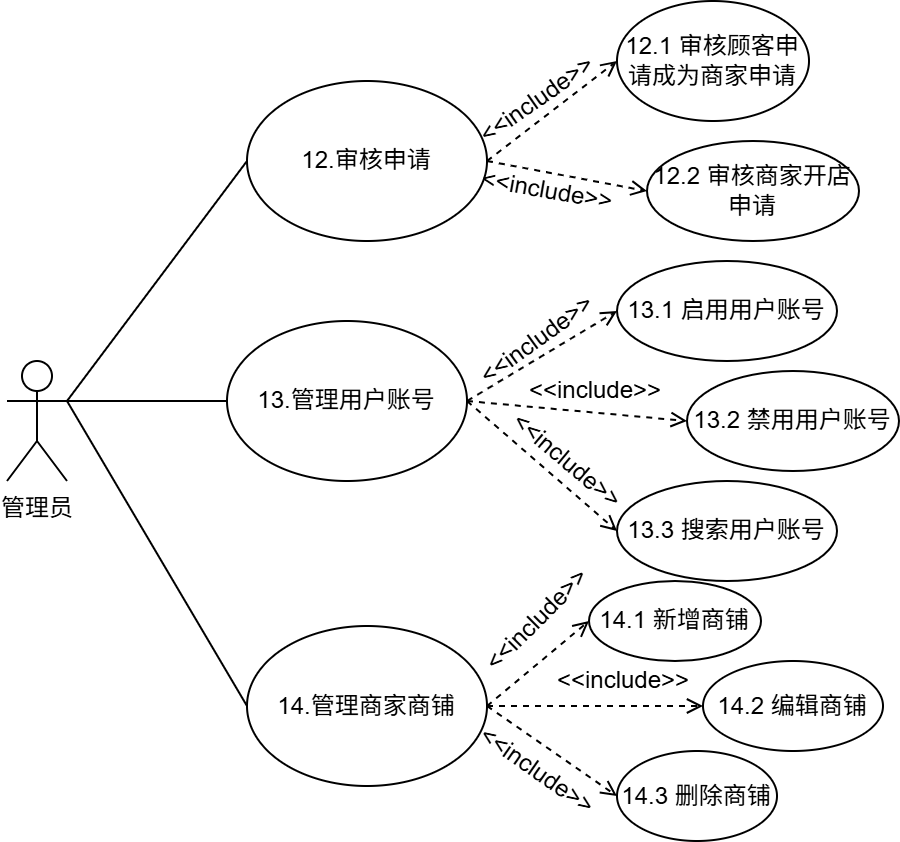
\includegraphics[width=4.99931in,height=4.67778in]{figures/srs/image16.png}
\caption{管理员用例图}
\changedfigure{需增加骑手审核、评价治理、活动监管、资产异常审计和平台数据看板。}
\end{figure}

\begin{longtable}[]{@{}
  >{\centering\arraybackslash}p{(\linewidth - 6\tabcolsep) * \real{0.1707}}
  >{\centering\arraybackslash}p{(\linewidth - 6\tabcolsep) * \real{0.2487}}
  >{\centering\arraybackslash}p{(\linewidth - 6\tabcolsep) * \real{0.1760}}
  >{\centering\arraybackslash}p{(\linewidth - 6\tabcolsep) * \real{0.3625}}@{}}
\caption{成为商家申请说明}\tabularnewline
\toprule\noalign{}
\endfirsthead
\endhead
\bottomrule\noalign{}
\endlastfoot
\textbf{编号} & 12.1 & \textbf{名称} & 审核顾客申请成为商家申请 \\
\textbf{执行者} & 管理员 & \textbf{优先级} & 高 \\
\textbf{描述} &
\multicolumn{3}{>{\raggedright\arraybackslash}p{(\linewidth - 6\tabcolsep) * \real{0.7871} + 4\tabcolsep}@{}}{%
管理员审核} \\
\textbf{前置条件} &
\multicolumn{3}{>{\raggedright\arraybackslash}p{(\linewidth - 6\tabcolsep) * \real{0.7871} + 4\tabcolsep}@{}}{%
无} \\
\textbf{基本流程} &
\multicolumn{3}{>{\raggedright\arraybackslash}p{(\linewidth - 6\tabcolsep) * \real{0.7871} + 4\tabcolsep}@{}}{%
\begin{minipage}[t]{\linewidth}\raggedright
\begin{quote}
进入用户审核列表，点击``审核''按钮，查看申请人详细信息
\end{quote}

选择``批准''或``拒绝''
\end{minipage}} \\
\textbf{结束状况} &
\multicolumn{3}{>{\raggedright\arraybackslash}p{(\linewidth - 6\tabcolsep) * \real{0.7871} + 4\tabcolsep}@{}}{%
\begin{minipage}[t]{\linewidth}\raggedright
\begin{quote}
顾客端``我的''页面的消息与通知出现新消息，通知审核结果；若管理员批准申请，顾客端``申请成为商家''按钮变为``切换到商家端''按钮
\end{quote}
\end{minipage}} \\
\textbf{可选流程} &
\multicolumn{3}{>{\raggedright\arraybackslash}p{(\linewidth - 6\tabcolsep) * \real{0.7871} + 4\tabcolsep}@{}}{%
-} \\
\textbf{异常流程} &
\multicolumn{3}{>{\raggedright\arraybackslash}p{(\linewidth - 6\tabcolsep) * \real{0.7871} + 4\tabcolsep}@{}}{%
-} \\
\textbf{备注} &
\multicolumn{3}{>{\raggedright\arraybackslash}p{(\linewidth - 6\tabcolsep) * \real{0.7871} + 4\tabcolsep}@{}}{%
-} \\
\end{longtable}

\begin{longtable}[]{@{}
  >{\centering\arraybackslash}p{(\linewidth - 6\tabcolsep) * \real{0.1707}}
  >{\centering\arraybackslash}p{(\linewidth - 6\tabcolsep) * \real{0.2106}}
  >{\centering\arraybackslash}p{(\linewidth - 6\tabcolsep) * \real{0.1428}}
  >{\centering\arraybackslash}p{(\linewidth - 6\tabcolsep) * \real{0.3927}}@{}}
\caption{审核商家开店申请说明}\tabularnewline
\toprule\noalign{}
\endfirsthead
\endhead
\bottomrule\noalign{}
\endlastfoot
\textbf{编号} & 12.2 & \textbf{名称} & 审核商家开店申请 \\
\textbf{执行者} & 管理员 & \textbf{优先级} & 高 \\
\textbf{描述} &
\multicolumn{3}{>{\raggedright\arraybackslash}p{(\linewidth - 6\tabcolsep) * \real{0.7461} + 4\tabcolsep}@{}}{%
管理员审核} \\
\textbf{前置条件} &
\multicolumn{3}{>{\raggedright\arraybackslash}p{(\linewidth - 6\tabcolsep) * \real{0.7461} + 4\tabcolsep}@{}}{%
无} \\
\textbf{基本流程} &
\multicolumn{3}{>{\raggedright\arraybackslash}p{(\linewidth - 6\tabcolsep) * \real{0.7461} + 4\tabcolsep}@{}}{%
进入商铺审核列表，点击``审核''按钮，查看商铺详细信息

选择``批准''或``拒绝''} \\
\textbf{结束状况} &
\multicolumn{3}{>{\raggedright\arraybackslash}p{(\linewidth - 6\tabcolsep) * \real{0.7461} + 4\tabcolsep}@{}}{%
\begin{minipage}[t]{\linewidth}\raggedright
\begin{quote}
顾客端``我的''页面的消息与通知出现新消息，通知审核结果；若管理员同意申请，商铺出现在商家商铺页面的已上线列表，否则出现在未通过列表
\end{quote}
\end{minipage}} \\
\textbf{可选流程} &
\multicolumn{3}{>{\raggedright\arraybackslash}p{(\linewidth - 6\tabcolsep) * \real{0.7461} + 4\tabcolsep}@{}}{%
-} \\
\textbf{异常流程} &
\multicolumn{3}{>{\raggedright\arraybackslash}p{(\linewidth - 6\tabcolsep) * \real{0.7461} + 4\tabcolsep}@{}}{%
-} \\
\textbf{备注} &
\multicolumn{3}{>{\raggedright\arraybackslash}p{(\linewidth - 6\tabcolsep) * \real{0.7461} + 4\tabcolsep}@{}}{%
-} \\
\end{longtable}

\begin{longtable}[]{@{}
  >{\centering\arraybackslash}p{(\linewidth - 6\tabcolsep) * \real{0.1707}}
  >{\centering\arraybackslash}p{(\linewidth - 6\tabcolsep) * \real{0.1629}}
  >{\centering\arraybackslash}p{(\linewidth - 6\tabcolsep) * \real{0.1448}}
  >{\centering\arraybackslash}p{(\linewidth - 6\tabcolsep) * \real{0.3514}}@{}}
\caption{启用用户账号说明}\tabularnewline
\toprule\noalign{}
\endfirsthead
\endhead
\bottomrule\noalign{}
\endlastfoot
\textbf{编号} & 13.1 & \textbf{名称} & 启用用户账号 \\
\textbf{执行者} & 管理员 & \textbf{优先级} & 高 \\
\textbf{描述} &
\multicolumn{3}{>{\raggedright\arraybackslash}p{(\linewidth - 6\tabcolsep) * \real{0.6591} + 4\tabcolsep}@{}}{%
管理员启用用户账号} \\
\textbf{前置条件} &
\multicolumn{3}{>{\raggedright\arraybackslash}p{(\linewidth - 6\tabcolsep) * \real{0.6591} + 4\tabcolsep}@{}}{%
无} \\
\textbf{基本流程} &
\multicolumn{3}{>{\raggedright\arraybackslash}p{(\linewidth - 6\tabcolsep) * \real{0.6591} + 4\tabcolsep}@{}}{%
管理员进入``用户管理''页面

对于已禁用用户，点击``启用''按钮} \\
\textbf{结束状况} &
\multicolumn{3}{>{\raggedright\arraybackslash}p{(\linewidth - 6\tabcolsep) * \real{0.6591} + 4\tabcolsep}@{}}{%
\begin{minipage}[t]{\linewidth}\raggedright
\begin{quote}
该用户状态由``已禁用''变为``已启用''，出现在已启用用户列表
\end{quote}
\end{minipage}} \\
\textbf{可选流程} &
\multicolumn{3}{>{\raggedright\arraybackslash}p{(\linewidth - 6\tabcolsep) * \real{0.6591} + 4\tabcolsep}@{}}{%
-} \\
\textbf{异常流程} &
\multicolumn{3}{>{\raggedright\arraybackslash}p{(\linewidth - 6\tabcolsep) * \real{0.6591} + 4\tabcolsep}@{}}{%
-} \\
\textbf{备注} &
\multicolumn{3}{>{\raggedright\arraybackslash}p{(\linewidth - 6\tabcolsep) * \real{0.6591} + 4\tabcolsep}@{}}{%
-} \\
\end{longtable}

\begin{longtable}[]{@{}
  >{\centering\arraybackslash}p{(\linewidth - 6\tabcolsep) * \real{0.1707}}
  >{\centering\arraybackslash}p{(\linewidth - 6\tabcolsep) * \real{0.2158}}
  >{\centering\arraybackslash}p{(\linewidth - 6\tabcolsep) * \real{0.1649}}
  >{\centering\arraybackslash}p{(\linewidth - 6\tabcolsep) * \real{0.2784}}@{}}
\caption{禁用用户账号说明}\tabularnewline
\toprule\noalign{}
\endfirsthead
\endhead
\bottomrule\noalign{}
\endlastfoot
\textbf{编号} & 13.2 & \textbf{名称} & 禁用用户账号 \\
\textbf{执行者} & 管理员 & \textbf{优先级} & 高 \\
\textbf{描述} &
\multicolumn{3}{>{\raggedright\arraybackslash}p{(\linewidth - 6\tabcolsep) * \real{0.6591} + 4\tabcolsep}@{}}{%
管理员禁用用户账号} \\
\textbf{前置条件} &
\multicolumn{3}{>{\raggedright\arraybackslash}p{(\linewidth - 6\tabcolsep) * \real{0.6591} + 4\tabcolsep}@{}}{%
无} \\
\textbf{基本流程} &
\multicolumn{3}{>{\raggedright\arraybackslash}p{(\linewidth - 6\tabcolsep) * \real{0.6591} + 4\tabcolsep}@{}}{%
管理员进入``用户管理''页面

对于已启用用户，点击``禁用''按钮} \\
\textbf{结束状况} &
\multicolumn{3}{>{\raggedright\arraybackslash}p{(\linewidth - 6\tabcolsep) * \real{0.6591} + 4\tabcolsep}@{}}{%
\begin{minipage}[t]{\linewidth}\raggedright
\begin{quote}
该用户状态由``已启用''变为``已禁用''，出现在已禁用用户列表
\end{quote}
\end{minipage}} \\
\textbf{可选流程} &
\multicolumn{3}{>{\raggedright\arraybackslash}p{(\linewidth - 6\tabcolsep) * \real{0.6591} + 4\tabcolsep}@{}}{%
-} \\
\textbf{异常流程} &
\multicolumn{3}{>{\raggedright\arraybackslash}p{(\linewidth - 6\tabcolsep) * \real{0.6591} + 4\tabcolsep}@{}}{%
-} \\
\textbf{备注} &
\multicolumn{3}{>{\raggedright\arraybackslash}p{(\linewidth - 6\tabcolsep) * \real{0.6591} + 4\tabcolsep}@{}}{%
-} \\
\end{longtable}

\begin{longtable}[]{@{}
  >{\centering\arraybackslash}p{(\linewidth - 6\tabcolsep) * \real{0.1728}}
  >{\centering\arraybackslash}p{(\linewidth - 6\tabcolsep) * \real{0.2147}}
  >{\centering\arraybackslash}p{(\linewidth - 6\tabcolsep) * \real{0.1649}}
  >{\centering\arraybackslash}p{(\linewidth - 6\tabcolsep) * \real{0.2795}}@{}}
\caption{搜索用户账号说明}\tabularnewline
\toprule\noalign{}
\endfirsthead
\endhead
\bottomrule\noalign{}
\endlastfoot
\textbf{编号} & 13.3 & \textbf{名称} & 搜索用户账号 \\
\textbf{执行者} & 管理员 & \textbf{优先级} & 高 \\
\textbf{描述} &
\multicolumn{3}{>{\raggedright\arraybackslash}p{(\linewidth - 6\tabcolsep) * \real{0.6591} + 4\tabcolsep}@{}}{%
管理员搜索用户账号} \\
\textbf{前置条件} &
\multicolumn{3}{>{\raggedright\arraybackslash}p{(\linewidth - 6\tabcolsep) * \real{0.6591} + 4\tabcolsep}@{}}{%
无} \\
\textbf{基本流程} &
\multicolumn{3}{>{\raggedright\arraybackslash}p{(\linewidth - 6\tabcolsep) * \real{0.6591} + 4\tabcolsep}@{}}{%
1.管理员进入``用户管理''页面

2. 在搜索栏搜索用户名、手机号或邮箱} \\
\textbf{结束状况} &
\multicolumn{3}{>{\raggedright\arraybackslash}p{(\linewidth - 6\tabcolsep) * \real{0.6591} + 4\tabcolsep}@{}}{%
得到模糊匹配结果} \\
\textbf{可选流程} &
\multicolumn{3}{>{\raggedright\arraybackslash}p{(\linewidth - 6\tabcolsep) * \real{0.6591} + 4\tabcolsep}@{}}{%
-} \\
\textbf{异常流程} &
\multicolumn{3}{>{\raggedright\arraybackslash}p{(\linewidth - 6\tabcolsep) * \real{0.6591} + 4\tabcolsep}@{}}{%
-} \\
\textbf{备注} &
\multicolumn{3}{>{\raggedright\arraybackslash}p{(\linewidth - 6\tabcolsep) * \real{0.6591} + 4\tabcolsep}@{}}{%
-} \\
\end{longtable}

\begin{longtable}[]{@{}
  >{\centering\arraybackslash}p{(\linewidth - 6\tabcolsep) * \real{0.1707}}
  >{\centering\arraybackslash}p{(\linewidth - 6\tabcolsep) * \real{0.1758}}
  >{\centering\arraybackslash}p{(\linewidth - 6\tabcolsep) * \real{0.1758}}
  >{\centering\arraybackslash}p{(\linewidth - 6\tabcolsep) * \real{0.3075}}@{}}
\caption{新增商铺说明}\tabularnewline
\toprule\noalign{}
\endfirsthead
\endhead
\bottomrule\noalign{}
\endlastfoot
\textbf{编号} & 14.1 & \textbf{名称} & 新增商铺 \\
\textbf{执行者} & 管理员 & \textbf{优先级} & 高 \\
\textbf{描述} &
\multicolumn{3}{>{\raggedright\arraybackslash}p{(\linewidth - 6\tabcolsep) * \real{0.6591} + 4\tabcolsep}@{}}{%
管理员新增商铺} \\
\textbf{前置条件} &
\multicolumn{3}{>{\raggedright\arraybackslash}p{(\linewidth - 6\tabcolsep) * \real{0.6591} + 4\tabcolsep}@{}}{%
无} \\
\textbf{基本流程} &
\multicolumn{3}{>{\raggedright\arraybackslash}p{(\linewidth - 6\tabcolsep) * \real{0.6591} + 4\tabcolsep}@{}}{%
管理员进入``商铺管理''页面

进入对应商家

点击``新增商铺''按钮

填写新商铺的图片、名称、地址、简介、类型} \\
\textbf{结束状况} &
\multicolumn{3}{>{\raggedright\arraybackslash}p{(\linewidth - 6\tabcolsep) * \real{0.6591} + 4\tabcolsep}@{}}{%
该商家商铺列表出现新增的商铺} \\
\textbf{可选流程} &
\multicolumn{3}{>{\raggedright\arraybackslash}p{(\linewidth - 6\tabcolsep) * \real{0.6591} + 4\tabcolsep}@{}}{%
-} \\
\textbf{异常流程} &
\multicolumn{3}{>{\raggedright\arraybackslash}p{(\linewidth - 6\tabcolsep) * \real{0.6591} + 4\tabcolsep}@{}}{%
-} \\
\textbf{备注} &
\multicolumn{3}{>{\raggedright\arraybackslash}p{(\linewidth - 6\tabcolsep) * \real{0.6591} + 4\tabcolsep}@{}}{%
-} \\
\end{longtable}

\begin{longtable}[]{@{}
  >{\centering\arraybackslash}p{(\linewidth - 6\tabcolsep) * \real{0.1707}}
  >{\centering\arraybackslash}p{(\linewidth - 6\tabcolsep) * \real{0.1776}}
  >{\centering\arraybackslash}p{(\linewidth - 6\tabcolsep) * \real{0.1741}}
  >{\centering\arraybackslash}p{(\linewidth - 6\tabcolsep) * \real{0.3075}}@{}}
\caption{编辑商铺说明}\tabularnewline
\toprule\noalign{}
\endfirsthead
\endhead
\bottomrule\noalign{}
\endlastfoot
\textbf{编号} & 14.2 & \textbf{名称} & 编辑商铺 \\
\textbf{执行者} & 管理员 & \textbf{优先级} & 高 \\
\textbf{描述} &
\multicolumn{3}{>{\raggedright\arraybackslash}p{(\linewidth - 6\tabcolsep) * \real{0.6591} + 4\tabcolsep}@{}}{%
管理员编辑商铺} \\
\textbf{前置条件} &
\multicolumn{3}{>{\raggedright\arraybackslash}p{(\linewidth - 6\tabcolsep) * \real{0.6591} + 4\tabcolsep}@{}}{%
无} \\
\textbf{基本流程} &
\multicolumn{3}{>{\raggedright\arraybackslash}p{(\linewidth - 6\tabcolsep) * \real{0.6591} + 4\tabcolsep}@{}}{%
管理员进入``商铺管理''页面

进入对应商家，找到对应商铺

点击``编辑''按钮

可编辑商铺图片、名称、地址、简介、类型} \\
\textbf{结束状况} &
\multicolumn{3}{>{\raggedright\arraybackslash}p{(\linewidth - 6\tabcolsep) * \real{0.6591} + 4\tabcolsep}@{}}{%
该商家商铺列表出现编辑后的商铺} \\
\textbf{可选流程} &
\multicolumn{3}{>{\raggedright\arraybackslash}p{(\linewidth - 6\tabcolsep) * \real{0.6591} + 4\tabcolsep}@{}}{%
-} \\
\textbf{异常流程} &
\multicolumn{3}{>{\raggedright\arraybackslash}p{(\linewidth - 6\tabcolsep) * \real{0.6591} + 4\tabcolsep}@{}}{%
-} \\
\textbf{备注} &
\multicolumn{3}{>{\raggedright\arraybackslash}p{(\linewidth - 6\tabcolsep) * \real{0.6591} + 4\tabcolsep}@{}}{%
-} \\
\end{longtable}

\begin{longtable}[]{@{}
  >{\centering\arraybackslash}p{(\linewidth - 6\tabcolsep) * \real{0.1707}}
  >{\centering\arraybackslash}p{(\linewidth - 6\tabcolsep) * \real{0.1792}}
  >{\centering\arraybackslash}p{(\linewidth - 6\tabcolsep) * \real{0.1814}}
  >{\centering\arraybackslash}p{(\linewidth - 6\tabcolsep) * \real{0.2985}}@{}}
\caption{删除商品说明}\tabularnewline
\toprule\noalign{}
\endfirsthead
\endhead
\bottomrule\noalign{}
\endlastfoot
\textbf{编号} & 14.3 & \textbf{名称} & 删除商铺 \\
\textbf{执行者} & 管理员 & \textbf{优先级} & 高 \\
\textbf{描述} &
\multicolumn{3}{>{\raggedright\arraybackslash}p{(\linewidth - 6\tabcolsep) * \real{0.6591} + 4\tabcolsep}@{}}{%
管理员删除商铺} \\
\textbf{前置条件} &
\multicolumn{3}{>{\raggedright\arraybackslash}p{(\linewidth - 6\tabcolsep) * \real{0.6591} + 4\tabcolsep}@{}}{%
无} \\
\textbf{基本流程} &
\multicolumn{3}{>{\raggedright\arraybackslash}p{(\linewidth - 6\tabcolsep) * \real{0.6591} + 4\tabcolsep}@{}}{%
管理员进入``商铺管理''页面

进入对应商家，找到对应商铺

点击``删除''按钮

确认删除} \\
\textbf{结束状况} &
\multicolumn{3}{>{\raggedright\arraybackslash}p{(\linewidth - 6\tabcolsep) * \real{0.6591} + 4\tabcolsep}@{}}{%
该商家商铺列表不再出现该商铺} \\
\textbf{可选流程} &
\multicolumn{3}{>{\raggedright\arraybackslash}p{(\linewidth - 6\tabcolsep) * \real{0.6591} + 4\tabcolsep}@{}}{%
-} \\
\textbf{异常流程} &
\multicolumn{3}{>{\raggedright\arraybackslash}p{(\linewidth - 6\tabcolsep) * \real{0.6591} + 4\tabcolsep}@{}}{%
-} \\
\textbf{备注} &
\multicolumn{3}{>{\raggedright\arraybackslash}p{(\linewidth - 6\tabcolsep) * \real{0.6591} + 4\tabcolsep}@{}}{%
-} \\
\end{longtable}

\input{body/srs_innovations}

\subsection{其他功能性需求}\label{ux5176ux4ed6ux529fux80fdux6027ux9700ux6c42}

首页提供搜索功能，用户可以搜索饿了么平台上的商铺；接入AI智能体，方便用户对商品的咨询；接入高德api，进行地理位置选择；首页轮播图展示销量前三的商铺；首页下方的综合排序按照商铺的评分（即商铺所获点赞数与收藏数加权归一的值）倒序排列；销量排序按照商铺的销量倒序排列；筛选可以按照是否免配送费、起送费的价格区间筛选相应的商铺。

\section{非功能性需求}\label{ux975eux529fux80fdux6027ux9700ux6c42}

\subsection{系统架构}\label{ux7cfbux7edfux67b6ux6784}

\begin{figure}[htbp]
\centering
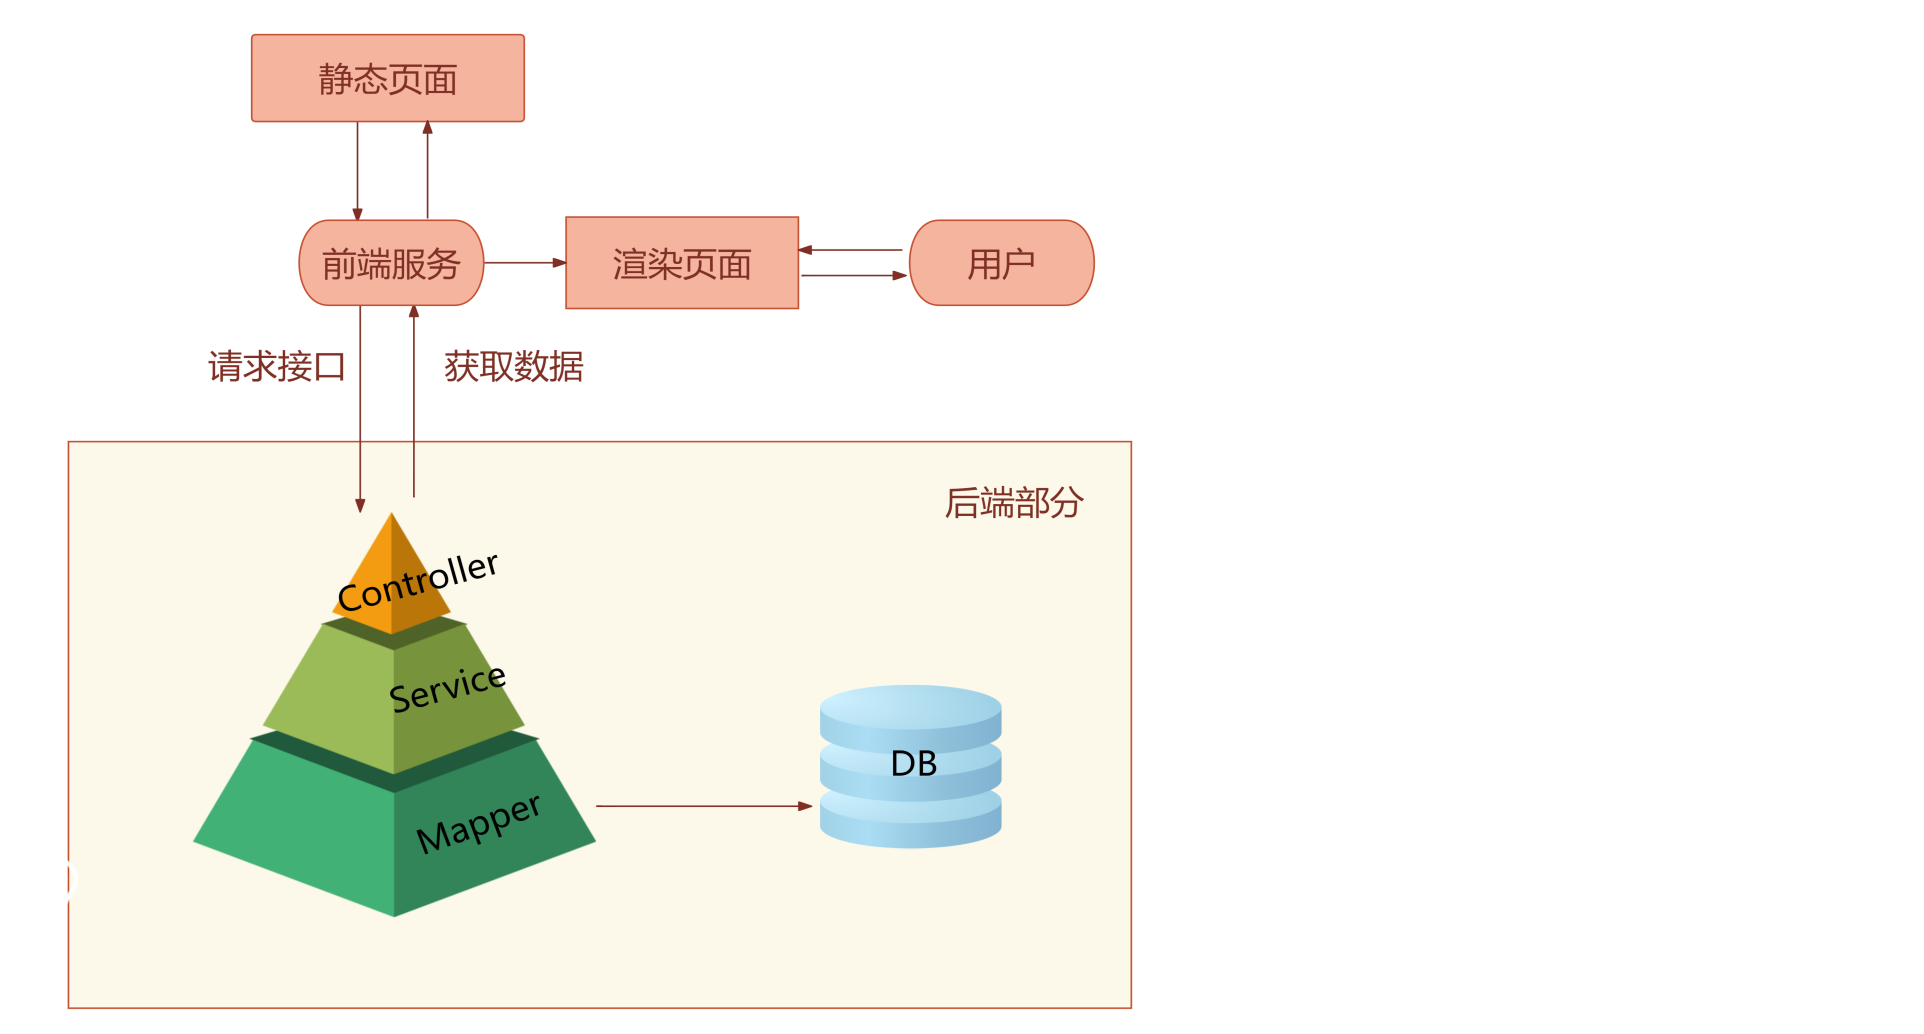
\includegraphics[width=2.95069in,height=2.60417in]{figures/srs/image17.png}
\caption{系统技术架构}
\changedfigure{需增加骑手端、\texttt{/api/v1} 网关、配送/资产/统计模块、第三方适配器、统一异常与自动化测试层。}
\end{figure}

\subsection{安全性}\label{ux5b89ux5168ux6027}

饿了么在前后端采用多种方案共同实现对于用户敏感信息的保护：

(1) 在传输密码时, 使用 HTTP POST 进行传输, 不在 URL中传输敏感数据

(2) 后端使用 SpringSecurity+JWT 实现用户登录和认证

(3) 用户注册时，后端利用 SpringSecurity 中的 BCryptPasswordEncoder
对密码进行加密处理之后再存入数据库，有效防止数据库被入侵后导致用户密码信息的泄露风险在前端,
我们在创建好的 axios 实例 axiosInstance 上，挂载两个拦截器

(4) 请求拦截器：

1. 前端向后端发送请求之前拦截

2. 在 header 添加 token，若有请求错误，在控制台打出

(5) 响应拦截器：

1. 后端向前端发送响应，前端接到之后拦截

2. 处理响应状态码错误 401，500 等

3. 网络错误，重试三次，重试失败，跳转回主页

4. 重试次数超过最大限制 3，跳转回主页

\input{body/srs_quality}
